\documentclass{lib/myskripsi}

\usepackage{blindtext}
\usepackage{longtable}

\renewcommand{\baselinestretch}{1.42}
\renewcommand{\UrlFont}{\small\rm}

%=============================================================================
% Package Daftar Pustaka, bentuk citasi
% Config
% - style, citestyle = {authoryear, numeric, apa, mla}
% - sorting {year,name,title} = ynt
%-----------------------------------------------------------------------------
\usepackage[
    backend=biber,
    style=authoryear,
    citestyle=authoryear,
    sorting=nty,
    giveninits=false,
    maxbibnames=3
    ]{biblatex}
\addbibresource{bibtex/daftar-pustaka.bib}
% new citation style
\let\oldcitate\cite
\newcommand*\thecite[1]{(\citeauthor{#1}, \citeyear{#1})}
%-----------------------------------------------------------------------------
% End Biblatex Config
%=============================================================================

%=============================================================================
% Definisi Data Peneliti, Judul, Pembimbing dan Penguji
%-----------------------------------------------------------------------------
\titleind{SISTEM IDENTIFIKASI KENDARAAN PADA PEMARKIRAN DENGAN PENGENALAN CITRA PELAT DAN PEMBACAAN RFID}

\fullname{MUH FIKRI SATRIA AMDANI}
\idnum{H131 16 501}

\examdate{\hspace{0.4cm} Februari 2021}

\degree{Sarjana Komputer}
\yearsubmit{2021}
\program{Sistem Informasi}
\dept{Matematika}
\faculty{Fakultas Matematika dan Ilmu Pengetahuan Alam}

\firstsupervisor{Dr. Eng. Armin Lawi, S.Si., M.Eng.}
\firstsupervisorNIP{19720423 199512 1 001}
\secondsupervisor{Musfira Putri Lukman, S.T., M.T.}
\secondsupervisorNIP{909048802}
\firstexaminer{ Dr. Hendra, S.Si., M.Kom.}
\secondexaminer{ Nur Hilal A Syahrir, S.Si., M.Si.}
%-----------------------------------------------------------------------------
% End Definisi Data Peneliti, Judul, Pembimbing dan Penguji
%=============================================================================

\begin{document}
    \noindent
    \textit{Seminar II}
    \coverproposal
    \pagenumbering{roman}

    %=============================================================================
    % Daftar isi, daftar gambar, daftar tabel
    %-----------------------------------------------------------------------------
    \tableofcontents
    \addcontentsline{toc}{chapter}{DAFTAR ISI}
    \newpage

    \listoftables
    \addcontentsline{toc}{chapter}{DAFTAR TABEL}
    \newpage

    \listoffigures
    \addcontentsline{toc}{chapter}{DAFTAR GAMBAR}
    \newpage
    %-----------------------------------------------------------------------------
    % End Daftar isi, daftar gambar, daftar tabel
    %=============================================================================

    \pagebreak
    \pagenumbering{arabic}

    %=============================================================================
    % Daftar masukan untuk Bab
    %-----------------------------------------------------------------------------
    \chapter{PENDAHULUAN}

\section{Latar Belakang}
Revolusi Industri merupakan periode di mana terjadinya perubahan secara besar-besaran di bidang pertanian, manufaktur, tekstil dan logam, pertambangan, transportasi, teknologi, dan sosial ekonomi \thecite{azli2017a}. Pada abad ke-18, mesin uap pertama ditemukan di Inggris. Mesin uap tersebut digunakan sebagai alat tenun mekanis pertama yang dapat meningkatkan produktivitas industri tekstil. Saat itu mesin uap mulai menggantikan peralatan kerja yang awalnya bergantung pada tenaga manusia dan hewan sekaligus memulai era revolusi industri pertama yang dikenal dengan Revolusi Industri 1.0. Revolusi industri kedua ditandai dengan penemuan tenaga listrik pada awal abad ke-20. Revolusi industri ketiga ditandai oleh mesin yang dapat bergerak dan berpikir secara otomatis, yaitu komputer dan robot \thecite{rahayu2019a}. 

Di abad ke-21 revolusi industry telah masuk ke era baru. Yakni telah berada pada revolusi industri keempat atau lebih dikenal dengan Revolusi Industri 4.0. Era ini telah mengubah banyak bidang kehidupan manusia, termasuk ekonomi, dunia kerja, bahkan gaya hidup. Revolusi industri 4.0 menawarkan teknologi cerdas yang dapat terhubung dengan berbagai bidang kehidupan manusia. Revolusi industri 4.0 menerapkan \textit{Internet of Things} (IoT) dan teknologi pada kegiatan analisis, manufaktur, robotik, komputasi canggih, \textit{artificial intellegence}, teknologi, kognitif, \textit{advance materials} dan \textit{augmented reality} dalam melaksanakan siklus operasi bisnis \thecite{suharman2019a}. Saat ini negara-negara di dunia mulai berkopetisi dalam pemanfaatan teknologi pada setiap sektor industrinya. Lalu bagaimana dengan indonesia ? Mempelajari konsep industri 4.0 untuk penerapannya di Indonesia menjadi suatu keharusan, sebab jika tidak maka industry dan manufaktur di Indonesia tidak akan dapat bersaing dengan industry dan manufaktur di negara-negara lain di dunia.

Revolusi industri 4.0 mencakup beragam teknologi canggih, seperti kecerdasan buatan (AI), \textit{wearables}, robotika canggih, \textit{3D printing}, dan \textit{Internet of Things} (IoT). \textit{Internet of Things} (IoT) adalah sekenario dari suatu objek yang dapat melakukan pengiriman data/informasi melalui jaringan tanpa campur tangan manusia \thecite{limantara2017a}. \textit{Konsep Internet of Things} sudah banyak digunakan dalam kehidupan sehari-hari di berbagai bidang, seperti bidang pertanian, bidang kesehatan, bidang industri, bidang keamanan, serta bidang transportasi.

Salah satu permasalahan yang banyak dijumpai diera sekarang adalah sistem parkir yang masih menggunakan metode konvensional untuk mencatat nomor pelat kendaraan yang akan parkir dan pembayaran yang masih menggunakan uang cash. Hal ini dapat memicu kemacetan, polusi udara dan suara, dan menambah tingkat stress pengendara. Untuk mengatasi masalah tersebut, dibuatlah suatu sistem dengan memanfaatkana konsep \textit{Internet of Things} di bidang transportasi dan keamanan. Sistem yang dimaksud adalah sistem parkir otomatis yang diletakkan di tempat khusus seperti di apartemen atau di perkantoran.

Salah satu aspek dalam sistem parkir otomatis adalah identifikasi citra pelat kendaraan untuk mendapatkan data nomor pelat tanpa campur tangan manusia. Identifikasi pelat kendaraan pada sistem parkir otomatis dapat dilakukan dengan kartu RFID dan pengolahan citra pelat kendaraan. Kemampuan RFID sebagai media pengenal secara nirkabel membuat RFID sering digunakan sebagai otorisasi untuk akses ruangan dan tempat, akan tetapi penggunaan RFID masih rentan terhadap keamanan akses. Penelitian ini menggabungkan identifikasi kartu RFID dan pembacaan citra pelat kendaraan sehingga dapat meningkatkan keamanan parkir dan dapat mempersingkat waktu pencatatan nomor pelat kendaraan yang masih bersifat konvensional.

\section{Rumusan Masalah}
Berdasarkan uraian pada latar belakang masalah diatas, dapat dikemukakan pertanyaan penelitian sebagai berikut:
\begin{enumerate}[topsep=0pt,itemsep=0pt,partopsep=0pt, parsep=0pt]
    \item Bagaimana cara merancang dan membangun sistem identifikasi kendaraan dengan pengenalan citra pelat dan pembacaan RFID ?
    \item Bagaimana cara membuat aplikasi web untuk memantau situasi lahan parkir ?
\end{enumerate}

\section{Batasan Masalah}
Batasan masalah pada penelitian ini adalah :
\begin{enumerate}[topsep=0pt,itemsep=0pt,partopsep=0pt, parsep=0pt]
    \item Alat yang dibuat bersifat prototype.
    \item Sistem parkir yang dibuat ditujukan untuk diterapkan di lingkungan berpenghuni tetap seperti apartemen atau perkantoran.
    \item Karakter pada pelat nomor harus sesuai dengan yang digunakan Samsat.
    \item Tidak melakukan analisis lebih lanjut pada deteksi nomor pelat kendaraan.
\end{enumerate}

\section{Tujuan Penelitian}
Berdasarkan rumusan masalah, maka tujuan penelitian ini adalah :
\begin{enumerate}[topsep=0pt,itemsep=0pt,partopsep=0pt, parsep=0pt]
    \item Merancang sistem identifikasi kendaraan dengan pengenalan citra pelat dan pembacaan RFID. 
    \item Membuat aplikasi web untuk memantau situasi lahan parkir.
    \item Menghubungkan sistem parkir dengan web yang dibuat sebagai \textit{user interface}.
\end{enumerate}

\section{Manfaat Penelitian}
Hasil penelitian ini diharapkan dapat bermanfaat :
\begin{enumerate}[topsep=0pt,itemsep=0pt,partopsep=0pt, parsep=0pt]
    \item Menghemat waktu dan bahan bakar.
    \item Terciptanya alat yang dapat menopang kemajuan industri.
    \item Mengurangi antrian Panjang yang disebabkan oleh pencatatan nomor pelat dan pembayaran parkir yang masih konvensional.
    \item Mempermudah pengelolah parkir untuk memantau sisa kapasitas lahan parkir yang tersedia.
    \item Membantu upaya pemerintah dalam pembangunan \textit{smart city} di Indonesia.
\end{enumerate}


    \chapter{TINJAUAN PUSTAKA}

\section{Internet of Things (IOT)}
\begin{afigure} 
    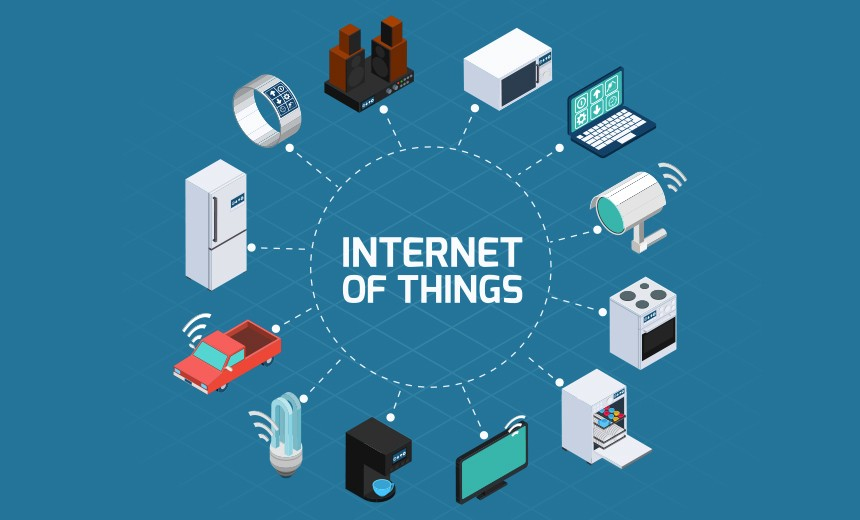
\includegraphics[width=0.85\textwidth, center]{images/iot.jpeg}
    \caption{Internet of Things}
    \label{fig:iot}
\end{afigure}

\textit{Internet of Things} adalah skenario dari suatu objek yang dapat melakukan suatu pengiriman data/informasi melalui jaringan tanpa campur tangan manusia. \textit{IoT} sangat erat hubungannya dengan komunikasi mesin ke mesin (M2M) tanpa campur tangan manusia ataupun komputer yang lebih dikenal dengan istilah cerdas \textit{(smart)} \thecite{limantara2017a}.

Cara Kerja \textit{Internet of Things} yaitu dengan memanfaatkan sebuah argumentasi pemrograman yang dimana tiap-tiap perintah argumennya itu menghasilkan sebuah interaksi antara sesama mesin yang terhubung secara otomatis tanpa campur tangan manusia dan dalam jarak berapa pun. Internetlah yang menjadi penghubung di antara kedua interaksi mesin tersebut, sementara manusia hanya bertugas sebagai pengatur dan pengawas bekerjanya alat tersebut secara langsung.Tantangan terbesar dalam mengkonfigurasi \textit{Internet of Things} ialah menyusun jaringan komunikasinya sendiri, yang dimana jaringan tersebut sangatlah kompleks, dan memerlukan sistem keamanan yang ketat. Selain itu biaya yang mahal sering menjadi penyebab kegagalan yang berujung pada gagalnya produksi.

Metode yang digunakan oleh \textit{Internet of Things} adalah nirkabel atau pengendalian secara otomatis tanpa mengenal jarak. Pengimplementasian \textit{Internet of Things} sendiri biasanya selalu mengikuti keinginan si developer dalam mengembangkan sebuah aplikasi yang ia ciptakan, apabila aplikasinya itu diciptakan guna membantu monitoring sebuah ruangan maka pengimplementasian \textit{Internet of Things} itu sendiri harus mengikuti alur diagram pemrograman mengenai sensor dalam sebuah rumah, berapa jauh jarak agar ruangan dapat dikontrol, dan kecepatan jaringan internet yang digunakan

Banyak manfaat yang didapatkan dari \textit{Internet of Things}. Pekerjaan yang kita lakukan menjadi cepat, mudah, dan efisien. Kemunculan \textit{Internet Of Things} \textit{(IoT)} memungkinkan perangkat komputer secara otomatis dapat melakukan kontrol terhadap suatu sistem dan memungkinkan pula untuk memberi aksi ke sistem terhadap kejadian yang terjadi pada sistem yang dikontrol secara realtime \thecite{ichwana2018a}.

\section{Automatic License Plate Recognition (ALPR)}
\textit{Automatic License Plate Recognition} adalah teknologi yang menggunakan pengenalan karakter pada gambar untuk membaca plat registrasi kendaraan. ALPR digunakan oleh polisi di beberapa negara di dunia untuk tujuan penegakan hukum, termasuk untuk memeriksa apakah kendaraan terdaftar atau tidak.

Pengenalan plat nomor otomatis dapat digunakan untuk menyimpan gambar yang diambil oleh kamera serta teks dari plat nomor. Umumnya sistem menggunakan pencahayaan inframerah untuk memungkinkan kamera mengambil gambar kapan saja, siang atau malam hari. Selain itu, teknologi ALPR juga harus memperhitungkan variasi nomor plat dari suatu negara karena bentuk dan ukuran nomor plat di satu negara dengan negara lainnya kemungkinan sangat berbeda.

ALPR menjadi tren baru dalam otomatisasi sistem transportasi. Pencatatan pelat nomor kendaraan bisa dilakukan tanpa campur tangan manusia. Meskipun teknologi tersebut telah ditetapkan di negara-negara maju, negara-negara berkembang seperti Indonesia belum menerapkan teknologi tersebut karena berbagai alasan \thecite{budianto2018a}.

\section{Raspberry Pi}
Raspberry Pi adalah komputer mini yang dirancang dan diproduksi di Inggris dengan tujuan awal untuk menyediakan perangkat komputasi yang murah untuk pendidikan. Raspberry Pi ditemukan pertama kali di University of Cambridge laboratory pada tahun 2006. Raspberry Pi dirilis secara komersial pada februari 2012. Sejak saat itu \textit{board} Raspberry Pi telah melalui sejumlah revisi dan tersedia dalam 2 model yaitu model A dan model B \thecite{wicaksono2018a}.

Secara kasar ditengah semua model Raspberry Pi terdapat sebuah semikonduktor persegi atau yang dikenal sebagai \textit{integrated circuit} atau \textit{chip}. \textit{Integrated Circuit} adalah \textit{sistem-on-chip} modul yang menyediakan kemampuan untuk pemrosesan umum \textit{(general purpose)}, render grafis, dan \textit{input/output} \thecite{wicaksono2018a}.

\begin{afigure} 
    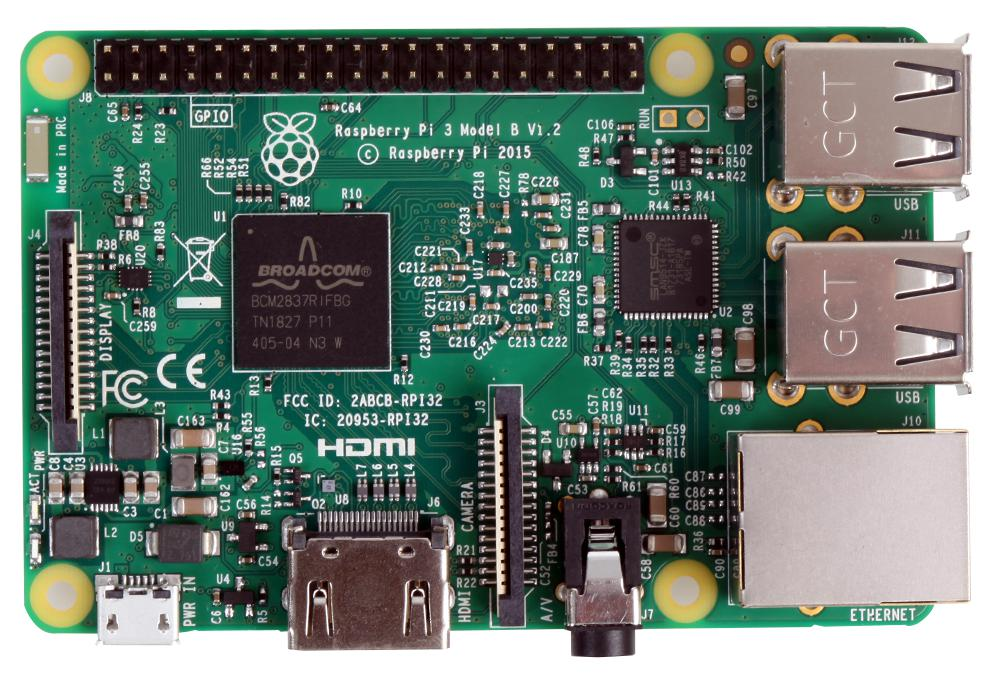
\includegraphics[width=0.85\textwidth, center]{images/raspberry pi 3b.jpg}
    \caption{Raspberry Pi model 3B}
    \label{fig:Raspberry3B}
\end{afigure}

Raspberry pi 3 adalah model terbaru Raspberry Pi. Raspberry Pi 3 menggunakan \textit{processor} terbaru yaitu Broadcom BCM283764 bit. BCM283764 lebih cepat dari pada BCM2836. Raspberry Pi 3 juga merupakan model pertama yang memiliki \textit{built-in wireless} (mampu terhubung ke jaringan WIFI dan juga memiliki perangkat \textit{Bluetooth}). Raspberry Pi model 3B bisa dilihat pada gambar ~\ref{fig:Raspberry3B}. Berikut merupakan spesifikasi dari Raspberry Pi 3 :

\begin{itemize}[topsep=0pt,itemsep=0pt,partopsep=0pt, parsep=0pt,]
    \item SoC: Broadcom BCM2837
    \item CPU: 4x ARM Cortex-A53, 1.2GHz
    \item GPU: Broadcom VideoCore IV
    \item RAM: 1GB LPDDR2 (900 MHz)
    \item Networking: 10/100 Ethernet, 2.4GHz 802.11n wireless
    \item Bluetooth: Bluetooth 4.1 Classic, Bluetooth Low Energy
    \item Storage: microSD
    \item GPIO: 40-pin header
    \item Ports: HDMI, 3.5mm analogue audio-video jack, 4x USB 2.0, Ethernet, CameraSerial Interface (CSI), Display Serial Interface (DSI)
\end{itemize}

\section{Module Sensor}
Sensor adalah sesuatu yang digunakan untuk mendeteksi adanya perubahan lingkungan fisik atau kimia.

\subsection{RFID MFRC522}
\textit{Radio Frequency Identification} (RFID) adalah teknologi untuk mengidentifkasi dan mengendalikan data dari jarak jauh menggunakan transmisi gelombang radio. RFID menggunakan sarana transponder atau RFID tag untuk menyimpan dan mengambil data dari jarak jauh. RFID tag mirip denganp penggunaan barcode yang melekat pada sebuah objek yang menyimpan identifikasi data obyek \thecite{singgeta2018a}.

RFID mempunyai 2 bagian komponen utama yang tak dapat dipisahkan, yaitu:
\begin{enumerate}[topsep=0pt,itemsep=0pt,partopsep=0pt, parsep=0pt]
    \item RFID Tag
    
    Merupakan sebuah perangkat yang akan diidentifikasi oleh RFID \textit{reader} yang dapat berupa perangkat pasif maupun aktif yang berisi suatu data atau informasi. Tag RFID, dapat berupa stiker, kertas atau plastik dengan beragam ukuran . Di dalam setiap tag ini terdapat chip yang mampu menyimpan sejumlah informasi tertentu. RFID Tag berfungsi sebagai transponder (transmitter dan responder) yang berisikan data dengan menggunakan frekuensi 125 KHz. RFID tag bisa dilihat pada gambar ~\ref{fig:rfidTag} 

    \begin{afigure} 
        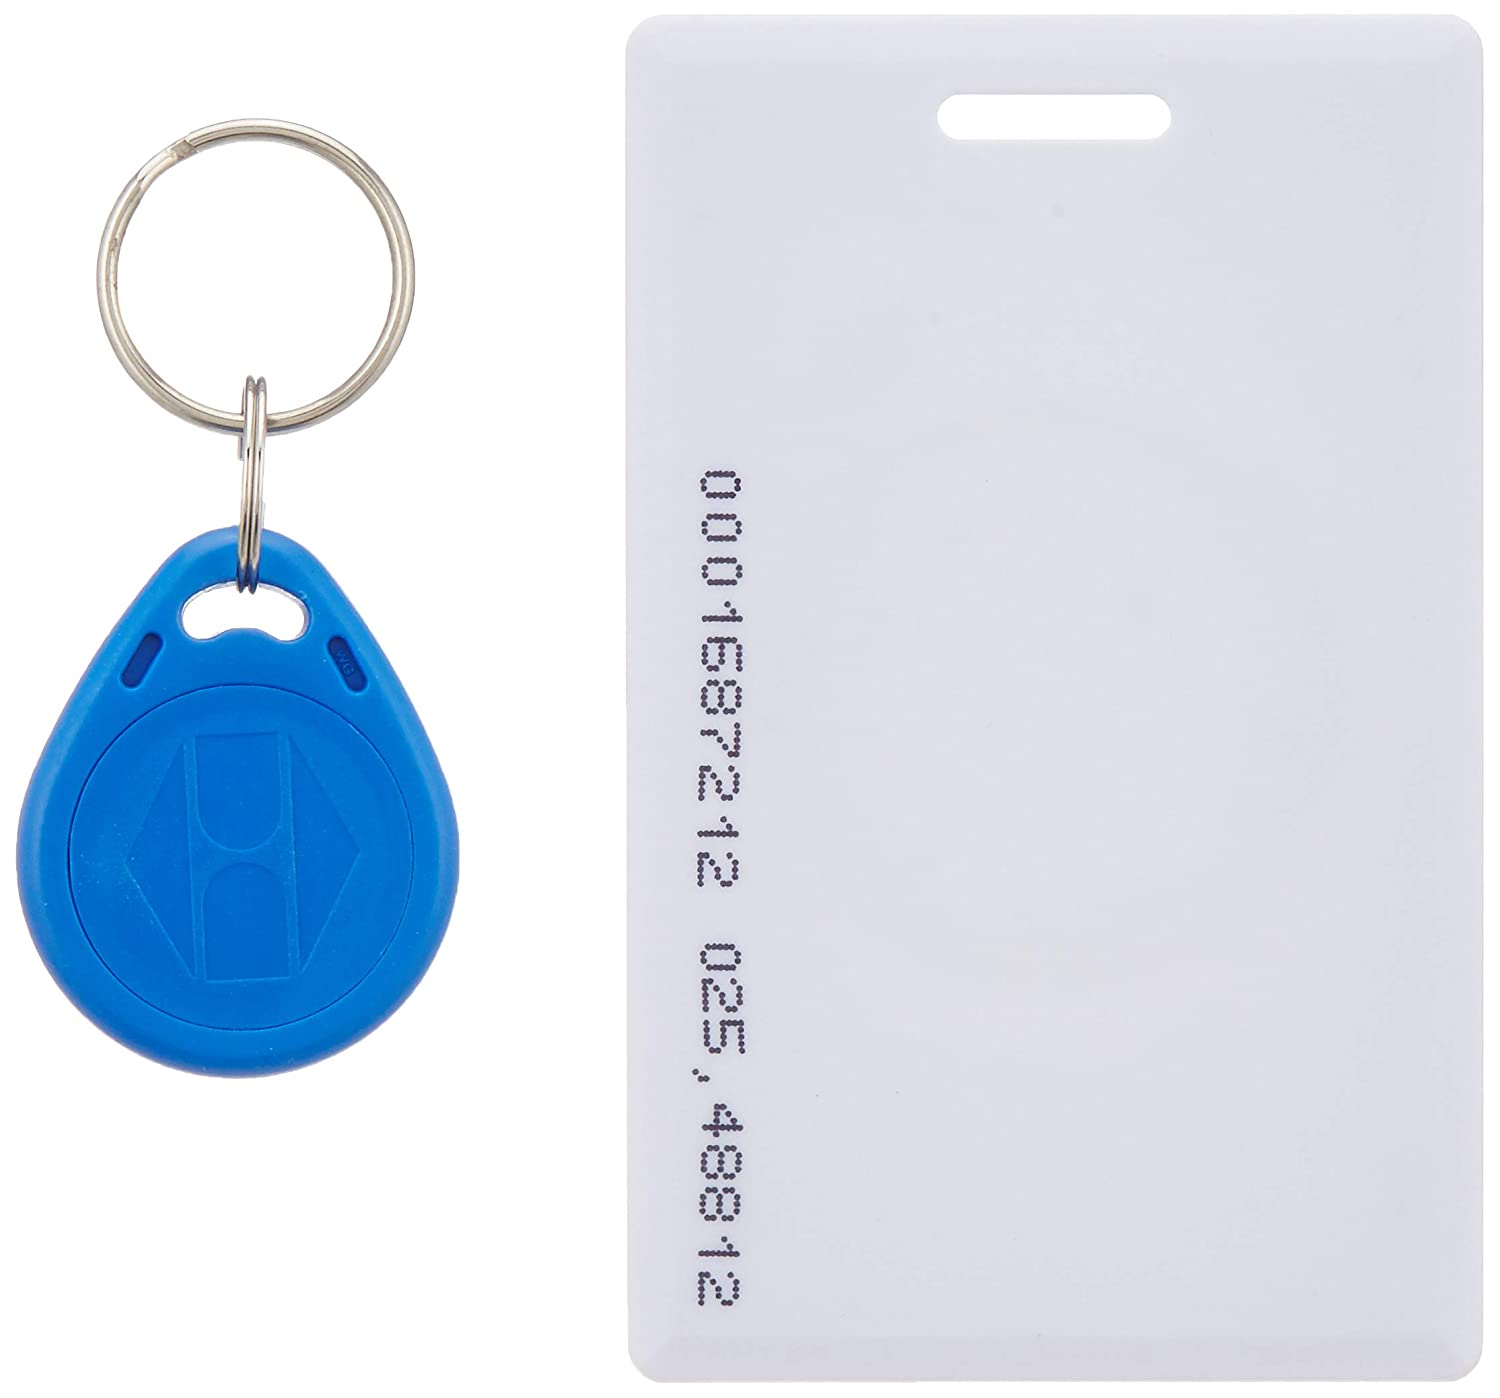
\includegraphics[width=0.85\textwidth, center]{images/rfidTag.jpg}
        \caption{RFID Tag}
        \label{fig:rfidTag}
    \end{afigure}

    Pada RFID tag terdapat 2 jenis yaitu \textit{Read-Write} dan \textit{Only Read}. Selain itu RFID tag mempunyai 2 komponen utama yang penting, antara lain:

    \begin{itemize}[topsep=0pt,itemsep=0pt,partopsep=0pt, parsep=0pt,]
        \item IC (\textit{Integrated Circuit}) : berfungsi sebagai pemproses informasi, modulasi serta demodulasi sinyal RF, yang beroperasi dengan catudaya DC.
        \item ANTENNA : mempunyai fungsi untuk mengirim maupun menerima sinyal RF.
    \end{itemize}

    \item RFID \textit{Reader}
    
    Berfungsi untuk membaca data dari RFID Tag. RFID \textit{Reader} dibedakan menjadi 2 macam, antara lain :
    \begin{itemize}[topsep=0pt,itemsep=0pt,partopsep=0pt, parsep=0pt,]
        \item Pasif : hanya bisa membaca data dari RFID tag aktif
        \item Aktif : dapat membaca data RFID tag pasif
    \end{itemize}
\end{enumerate}

\subsection{HC-SR04}
Sensor ultrasonik adalah sebuah sensor yang mengubah besaran fisis berupa bunyi menjadi besaran listrik dan sebaliknya. Cara kerja sensor ini didasarkan pada prinsip dari pantulan suatu gelombang suara sehingga dapat dipakai untuk menafsirkan jarak suatu benda dengan frekuensi tertentu. Disebut sebagai sensor ultrasonik karena sensor ini menggunakan gelombang ultrasonik (bunyi ultrasonik). Bunyi ultrasonik bisa merambat melalui zat padat, cair dan gas. Reflektivitas bunyi ultrasonik di permukaan zat padat hampir sama dengan reflektivitas bunyi ultrasonik di permukaan zat cair. Akan tetapi, gelombang bunyi ultrasonik akan diserap oleh tekstil dan busa.

\begin{afigure} 
    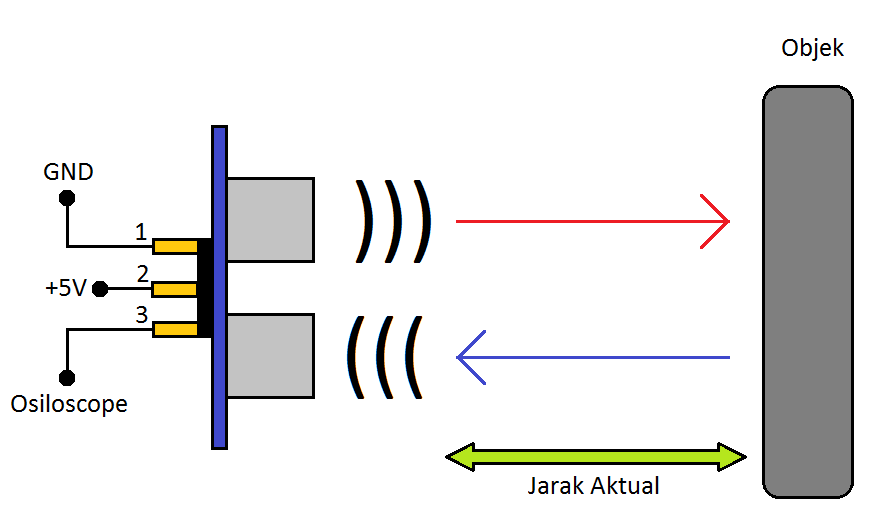
\includegraphics[width=0.85\textwidth, center]{images/cara kerja ultrasonik.png}
    \caption{Cara Kerja Sensor Ultrasonik}
    \label{fig:caraKerjaUltrasonic}
\end{afigure}

Secara umum, alat ini akan menembakkan gelombang ultrasonik menuju suatu area atau suatu target. Setelah gelombang menyentuh permukaan target, maka target akan memantulkan kembali gelombang tersebut. Gelombang pantulan dari target akan ditangkap oleh sensor, kemudian sensor menghitung selisih antara waktu pengiriman gelombang dan waktu gelombang pantul diterima \thecite{limantara2017a}. Ilustrasinya bisa dilihat pada gambar ~\ref{fig:caraKerjaUltrasonic}.

\begin{figure} [H]
    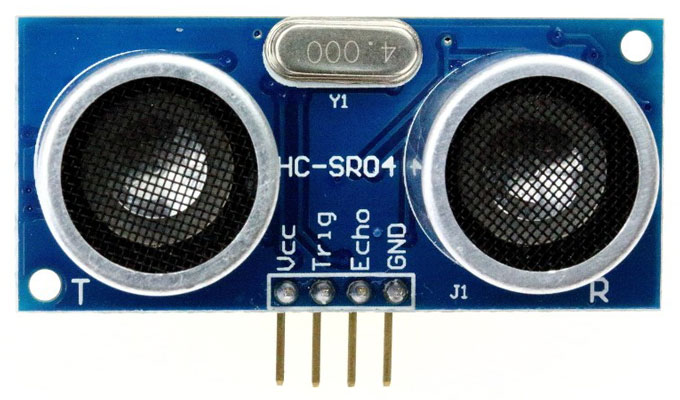
\includegraphics[width=0.85\textwidth, center]{images/ultrasonik.jpg}
    \caption{Sensor Ultrasonik}
    \label{fig:SensorUltrasonicHC-SR04}
\end{figure}

HC-SR04 merupakan sensor ultrasonik yang berfungsi sebagai pengirim, penerima, dan pengontrol gelombang ultrasonik. Alat ini bisa digunakan untuk mengukur jarak benda dari 2cm-4m dengan akurasi 3mm. Alat ini memiliki 4 pin, pin Vcc, Gnd, Trigger, dan Echo. Pin Vcc untuk listrik positif dan Gnd untuk ground-nya. Pin Trigger untuk trigger keluarnya sinyal dari sensor dan pin Echo untuk menangkap sinyal pantul dari benda. Sensor ultrasonik HC-SR04 bisa dilihat pada gambar ~\ref{fig:SensorUltrasonicHC-SR04}.

\subsection{SG90}
SG90 adalah sebuah servo kecil dengan output power yang tinggi. Motor ini dapat berotasi sekitar 180 derajat dan bisa bekerja seperti servo lainnya hanya saja ukurannya lebih kecil \thecite{wicaksono2018a}.

\begin{figure} [H]
    % 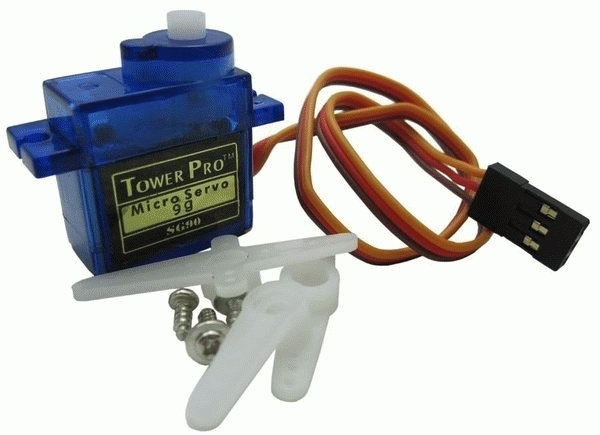
\includegraphics[width=0.85\textwidth, center]{images/servo.jpg}
    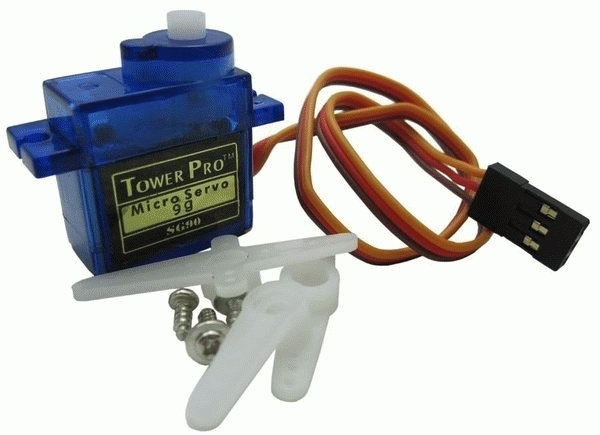
\includegraphics[width=0.50\textwidth, center]{images/servo.jpg}
    \caption{Servo SG90}
    \label{fig:servo}
\end{figure}

Gambar ~\ref{fig:servo} merupakan gambar dari servo SG90.

\subsection{Kamera Raspberry Pi v2}
Modul Kamera v2 memiliki sensor Sony IMX219 8-megapiksel. Modul Kamera dapat digunakan untuk mengambil video definisi tinggi, dan juga foto. Gambar ~\ref{fig:raspicamera} merupakan gambar dari kamera Raspberry Pi.

\begin{afigure} 
    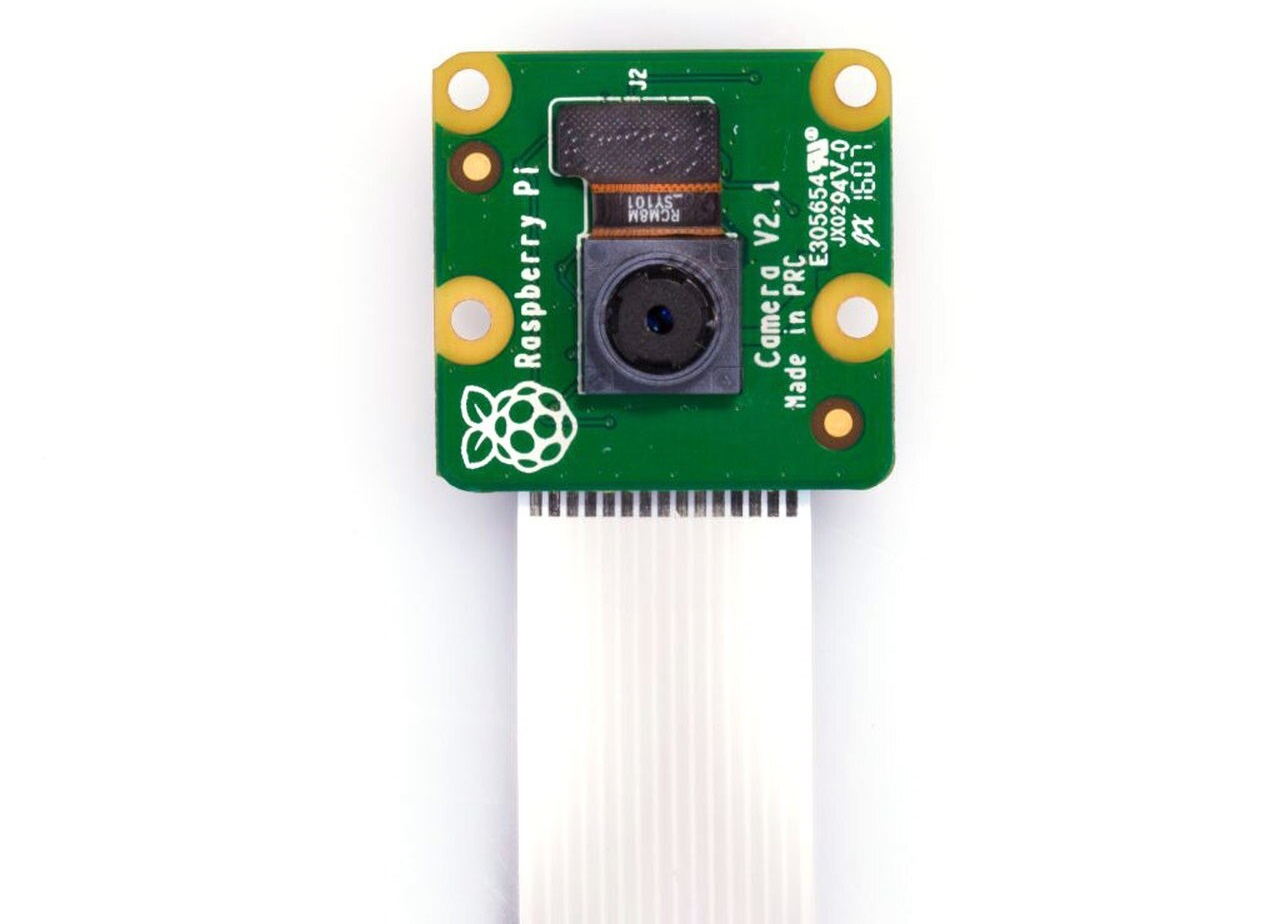
\includegraphics[width=0.85\textwidth, center]{images/raspicamera.jpg}
    \caption{ Kamera Raspberry Pi}
    \label{fig:raspicamera}
\end{afigure}

\subsection{API, REST API, dan RESTful API}


    \chapter{METODE PENENILITIAN}

\setlength{\intextsep}{0cm}
% \setlength{\textfloatsep}{-1cm}

\section{Waktu dan Lokasi Penelitian}
Penelitian ini dilaksanakan dari bulan juli 2020 sampai dengan bulan november 2020. Lokasi penelitian dilakukan di Laboratorium Rekayasa Perangkat Lunak Fakultas Matematika dan Ilmu Pengetahuan Alam, Universitas Hasanuddin.

\section{Tahapan Penelitian}

\begin{table} [H]
    \begin{tabular}{|>{\centering\arraybackslash}m{1\linewidth} |}
        \hline
        \textbf{Analisis Kebutuhan}\\ 
        Pada tahapan ini merupakan tahap awal yaitu menganalisis semua kebutuhan yang diperlukan selama meneliti seperti pengumpulan teori terkait dengan penelitian yang terdapat dalam buku atau jurnal.\\
        \hline
    \end{tabular}
\end{table}

\begin{center}
    \bigg\downarrow
\end{center}

\begin{table} [H]
    \begin{tabular}{|>{\centering\arraybackslash}m{1\linewidth} |}
        \hline
        \textbf{Desain Sistem}\\ 
        Pada tahap ini dilakukan perancangan sistem yang akan dibangun seperti, rancangan sistem, rancangan skematik alat, \textit{use case} diagram, \textit{activity} diagram dan perancangan aplikasi web.\\
        \hline
    \end{tabular}
\end{table}

\begin{center}
    \bigg\downarrow
\end{center}

\begin{table} [H]
    \begin{tabular}{|>{\centering\arraybackslash}m{1\linewidth} |}
        \hline
        \textbf{Implementasi}\\ 
        Pada tahapan ini dilakukan implementasi dari hasil perancangan pada tahapan sebelumnya. Di tahapan inilah pembangunan sistem parkir, perangkaian sensor-sensor dan \textit{microcontoller} dilakukan.\\
        \hline
    \end{tabular}
\end{table}

\begin{center}
    \bigg\downarrow
\end{center}

\begin{table} [H]
    \begin{tabular}{|>{\centering\arraybackslash}m{1\linewidth} |}
        \hline
        \textbf{Pengujian Sistem}\\ 
        Pada tahapan ini hasil dari pembuatan sistem siap untuk diimplementasikan. Sensor ditempatkan di tempat yang sudah disediakan, maka alat ini akan mengumpulkan data yang dibutuhkan seperti nomor plat, id rfid, dan jarak ultrasonik. Data yang berhasil dikumpulkan akan disimpan di database dan bisa dilihat di web.\\
        \hline
    \end{tabular}
\end{table}

\begin{center}
    \bigg\downarrow
\end{center}

\begin{table} [H]
    \begin{tabular}{|>{\centering\arraybackslash}m{1\linewidth} |}
        \hline
        \textbf{Kesimpulan}\\ 
        Pada tahap ini merupakan tahap penting terakhir dari penelitian ini. Pada tahapan ini hasil dari pembuatan sistem parkir sudah siap untuk diimplementasikan.\\
        \hline
    \end{tabular}
\end{table}

\section{Sumber Data}
Sumber data dari penelitian ini menggunakan data primer yang didapatkan secara langsung dari sensor yang digunakan dalam sistem parkir.

\section{Rancangan Sistem}
Sensor dan kamera akan terhubung dengan raspberry pi. Berikut ini adalah gambaran mengenai rancangan dari penelitian ini :

\begin{afigure} 
    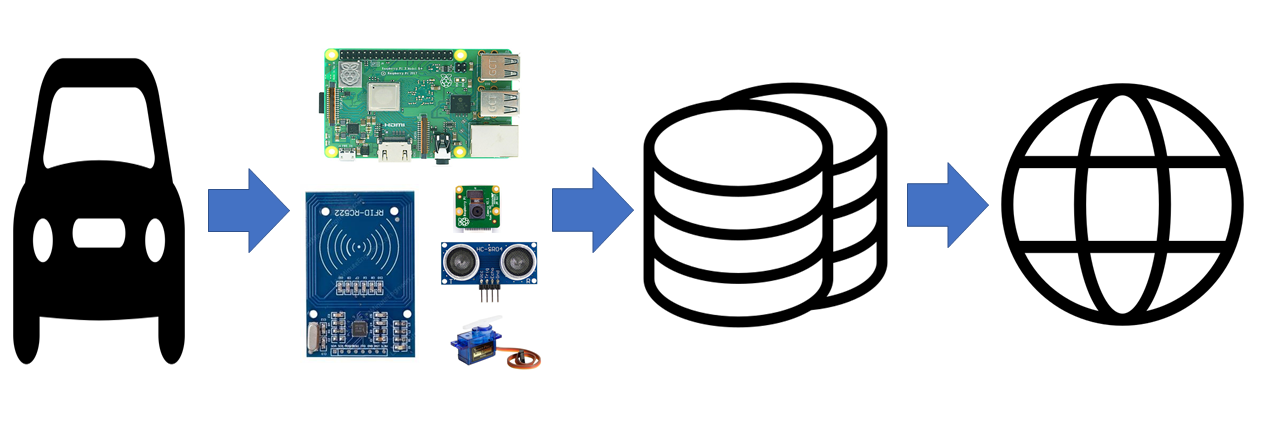
\includegraphics[width=0.85\textwidth, center]{images/rancangan sistem.png}
    \caption{Rancangan Sistem}
    \label{fig:RancanganSistem}
\end{afigure}

Pada gambar ~\ref{fig:RancanganSistem} saat pengemudi kendaraan menempelkan tag RFID mereka ke RFID reader, kamera pada raspberry akan mengambil gambar untuk di identifikasi nomor pelat tersebut. Hasil identifikasi akan berupa data nomor pelat kendaraan yang akan disimpan. Setelah itu servo yang berfungsi sebagai palang pintu akan terbuka. Data yang dikumpulkan oleh sensor berupa Id RFID dan nomor pelat kendaraan dapat dilihat melalui aplikasi web.

\section{Rancangan \textit{Use Case} Diagram}
Rancangan \textit{use case} diagram pada penelitian ini dapat di gambarkan seperti diagram dibawah ini:

\begin{afigure} 
    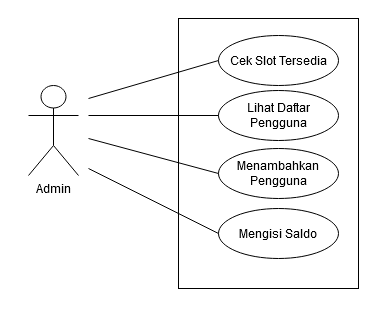
\includegraphics[width=0.85\textwidth, center]{images/Use Case Diagram.png}
    \caption{Use Case Diagram}
    \label{fig:usecasediagram}
\end{afigure}

sesuai dengan gambar ~\ref{fig:usecasediagram}, sistem yang akan dibangun hanya terdapat satu jenis akun yaitu akun admin yang akan mengawasi seluruh aktivitas pemarkiran melalui aplikasi web sebagai \textit{user interface}.

\section{Instrumen Penelitian}
Instrumen penelitian pada penelitian ini meliputi kebutuhan perangkat keras dan kebutuhan perangkat lunak.

\begin{enumerate}[topsep=0pt,itemsep=0pt,partopsep=0pt, parsep=0pt]
\item Kebutuhan perangkat keras
    \begin{itemize}[topsep=0pt,itemsep=0pt,partopsep=0pt, parsep=0pt,]
        \item Raspberry Pi
        \item Sensor RFID MFRC522
        \item Sensor Ultrasonik HC-SR04
        \item Servo SG90
        \item Camera Raspberry Pi v2 8mp
        \item Kabel Jumper
        \item Bread Board
        \item Memori Card
    \end{itemize}
\item Kebutuhan perangkat lunak
    \begin{itemize}[topsep=0pt,itemsep=0pt,partopsep=0pt, parsep=0pt,]
        \item \textit{Operating System (OS)} Raspbian
        \item \textit{Python Programming Language} (bahasa pemrograman yang digunakan)
        \item Visual Studio Code
        \item Web Browser
    \end{itemize}
\end{enumerate}
    \chapter{HASIL DAN PEMBAHASAN}

\section{Hasil Rancangan Sistem Identifikasi Kendaraan Pada Pemarkiran Dengan Pengenalan Citra Dan Pembacaan RFID}

\subsection{Hasil Perancangan Perangkat Keras}
\begin{figure} [H]
    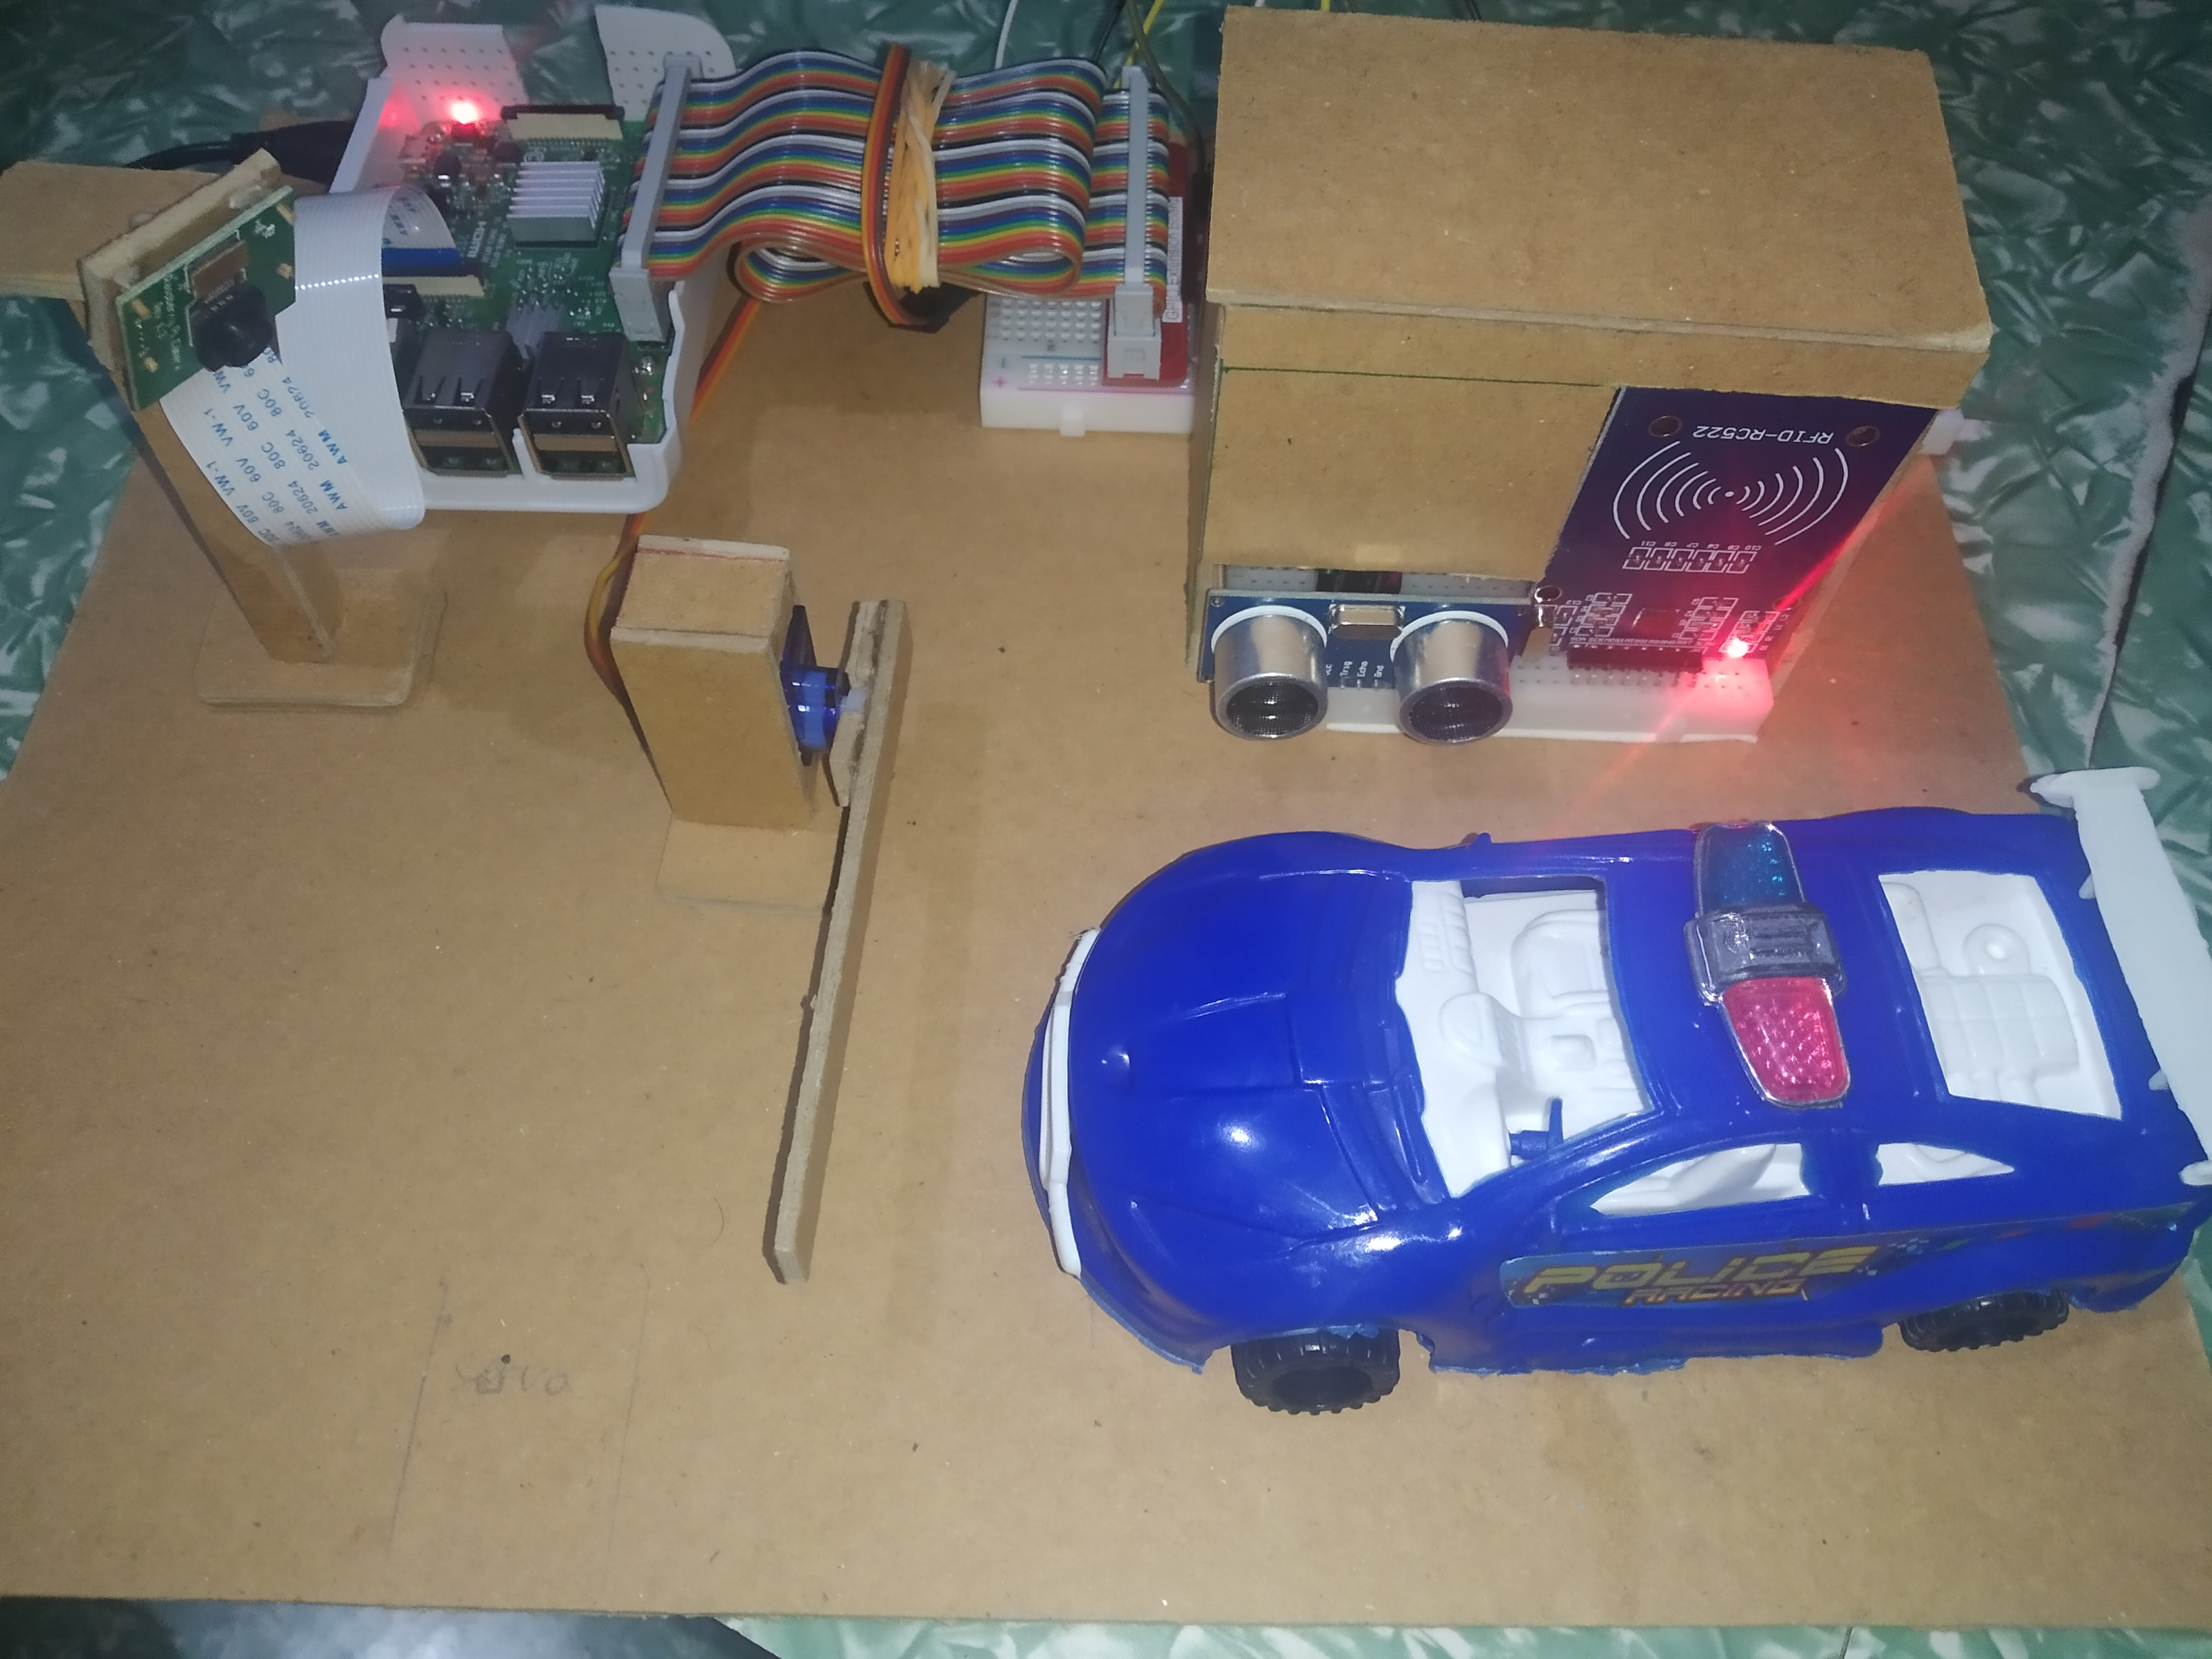
\includegraphics[height=7cm, width=0.5\textwidth, center]{images/alat-full-mobil.jpg}
    \caption{Hasil Rancangan dan Pemasangan Alat}
    \label{fig:alatfullmobil}
\end{figure}

\begin{figure} [H]
    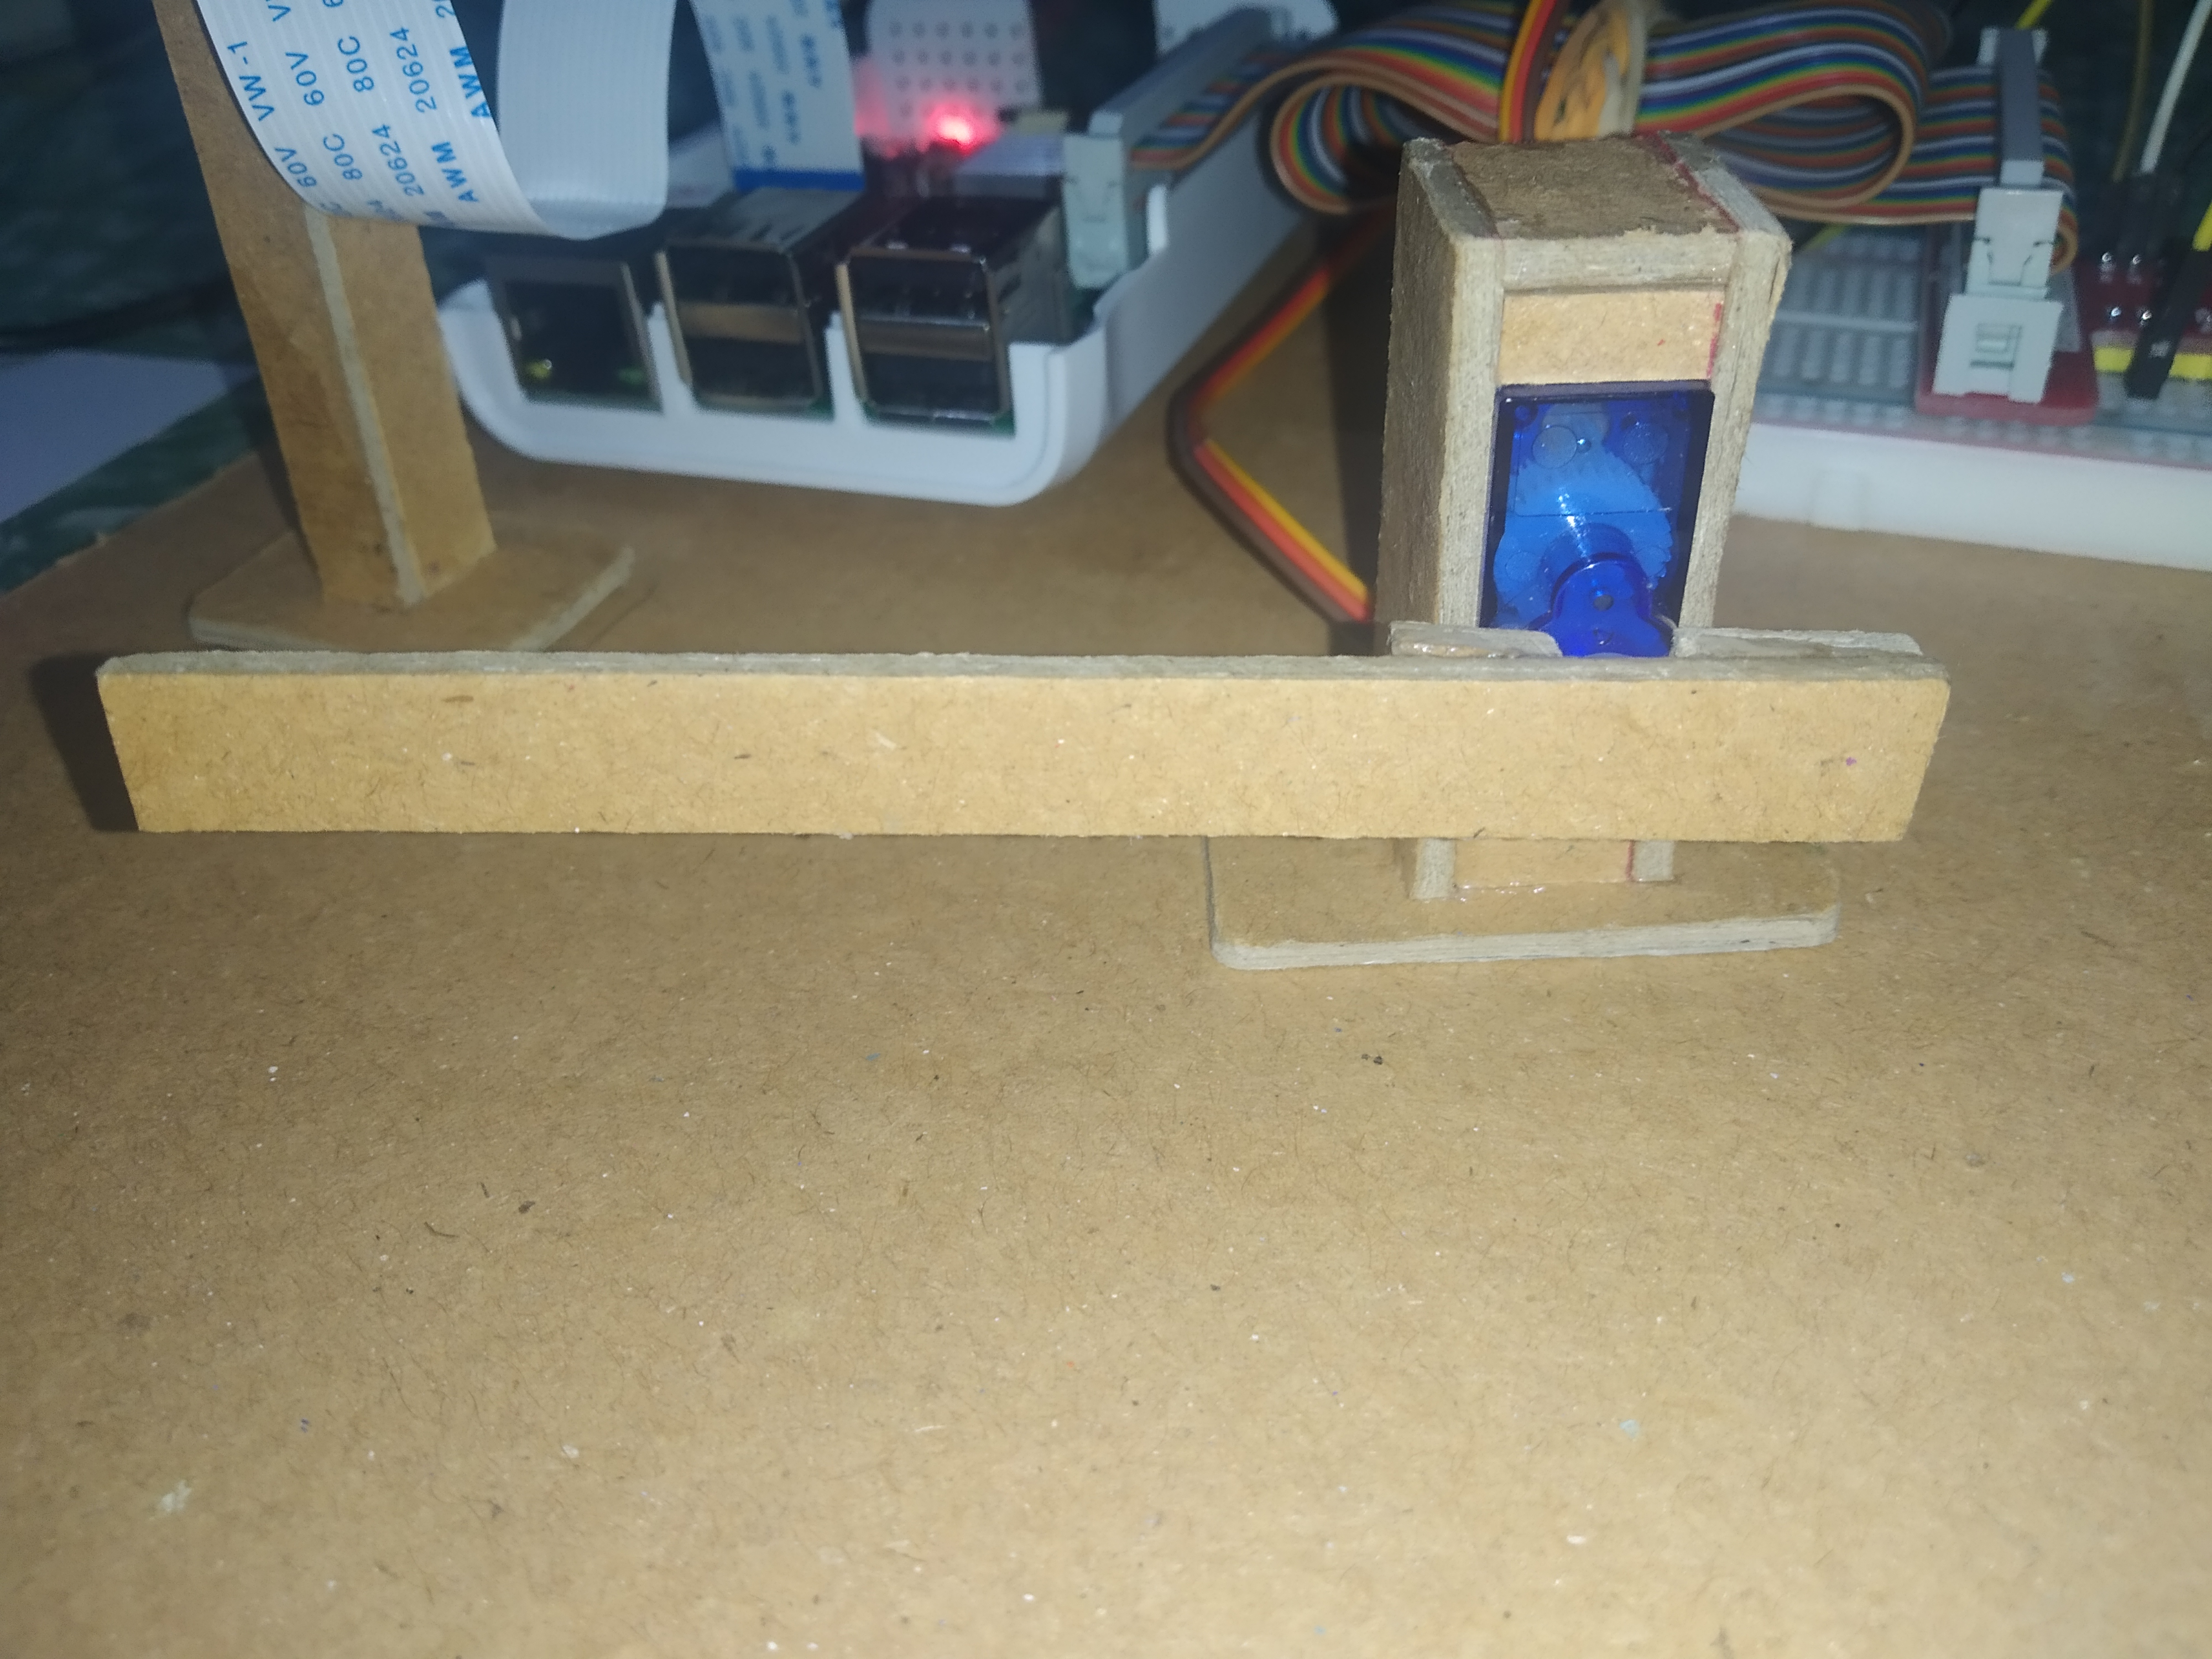
\includegraphics[height=7cm, width=0.5\textwidth, center]{images/alat-servo.jpg}
    \caption{Hasil Rancangan Servo}
    \label{fig:alatservo}
\end{figure}

\begin{figure} [H]
    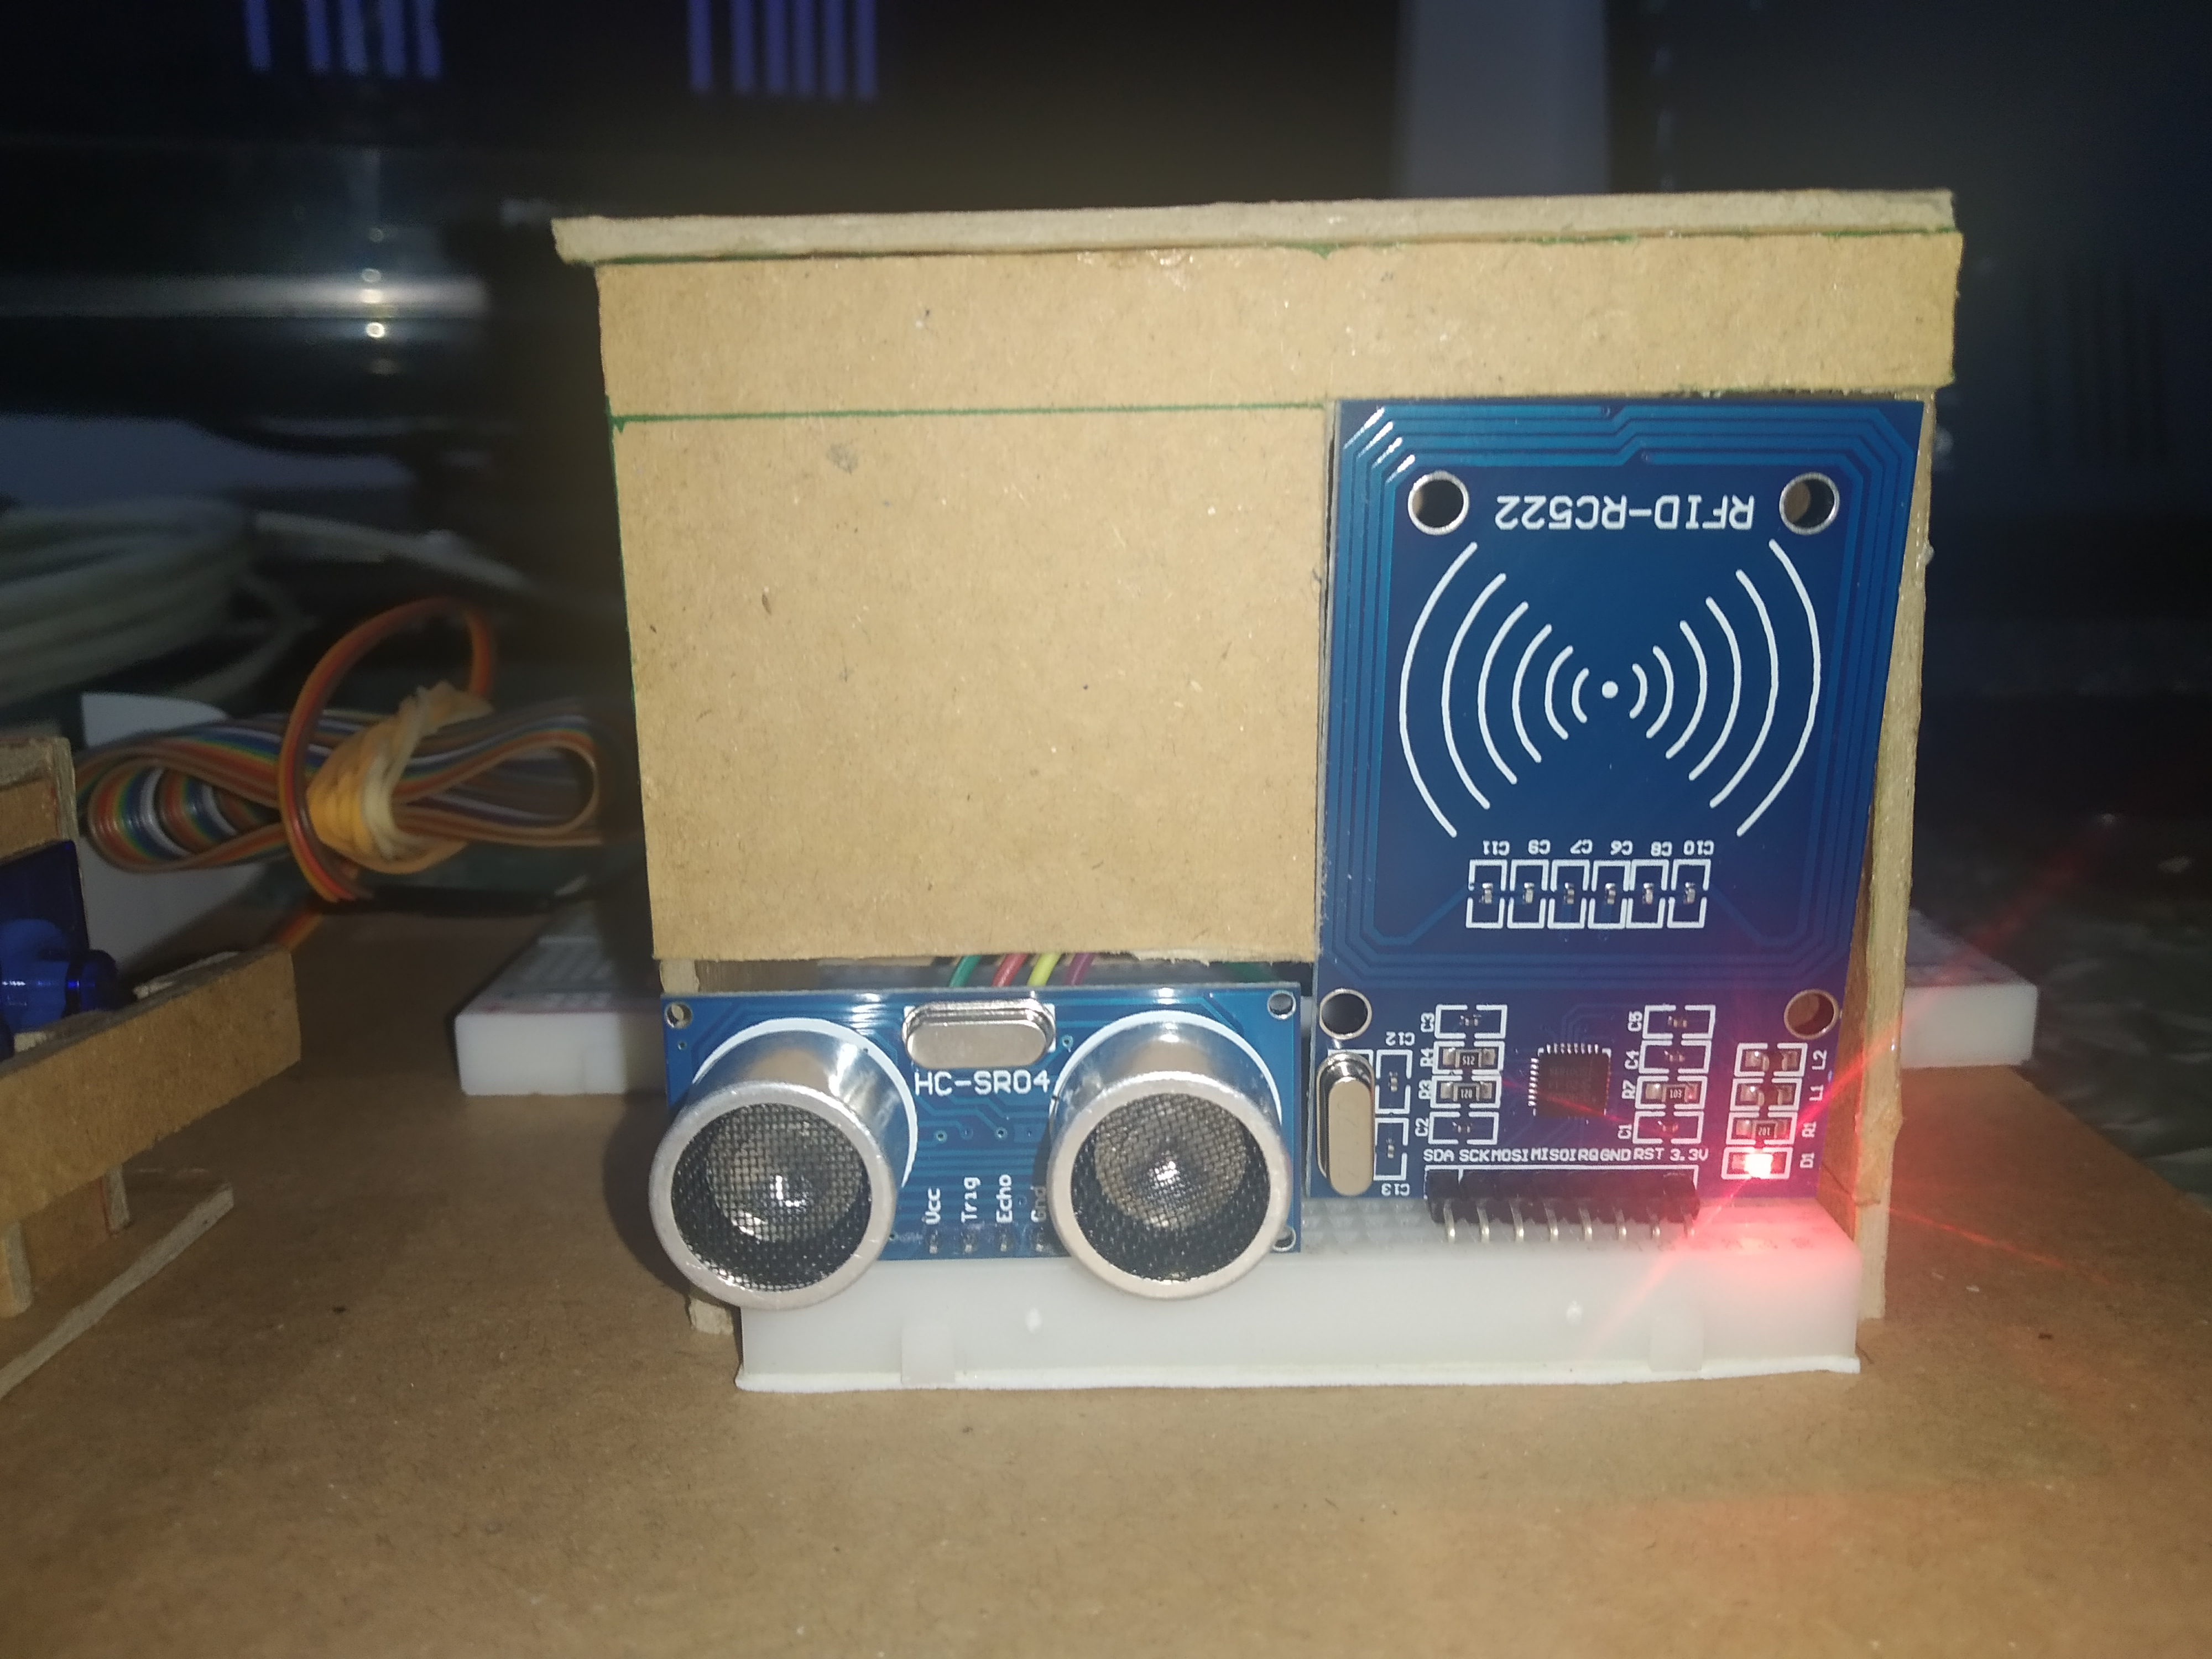
\includegraphics[height=7cm, width=0.5\textwidth, center]{images/alat-ultra&rfid.jpg}
    \caption{Hasil Rancangan Ultrasonik dan RFID}
    \label{fig:alatultrarfid}
\end{figure}

\begin{figure} [H]
    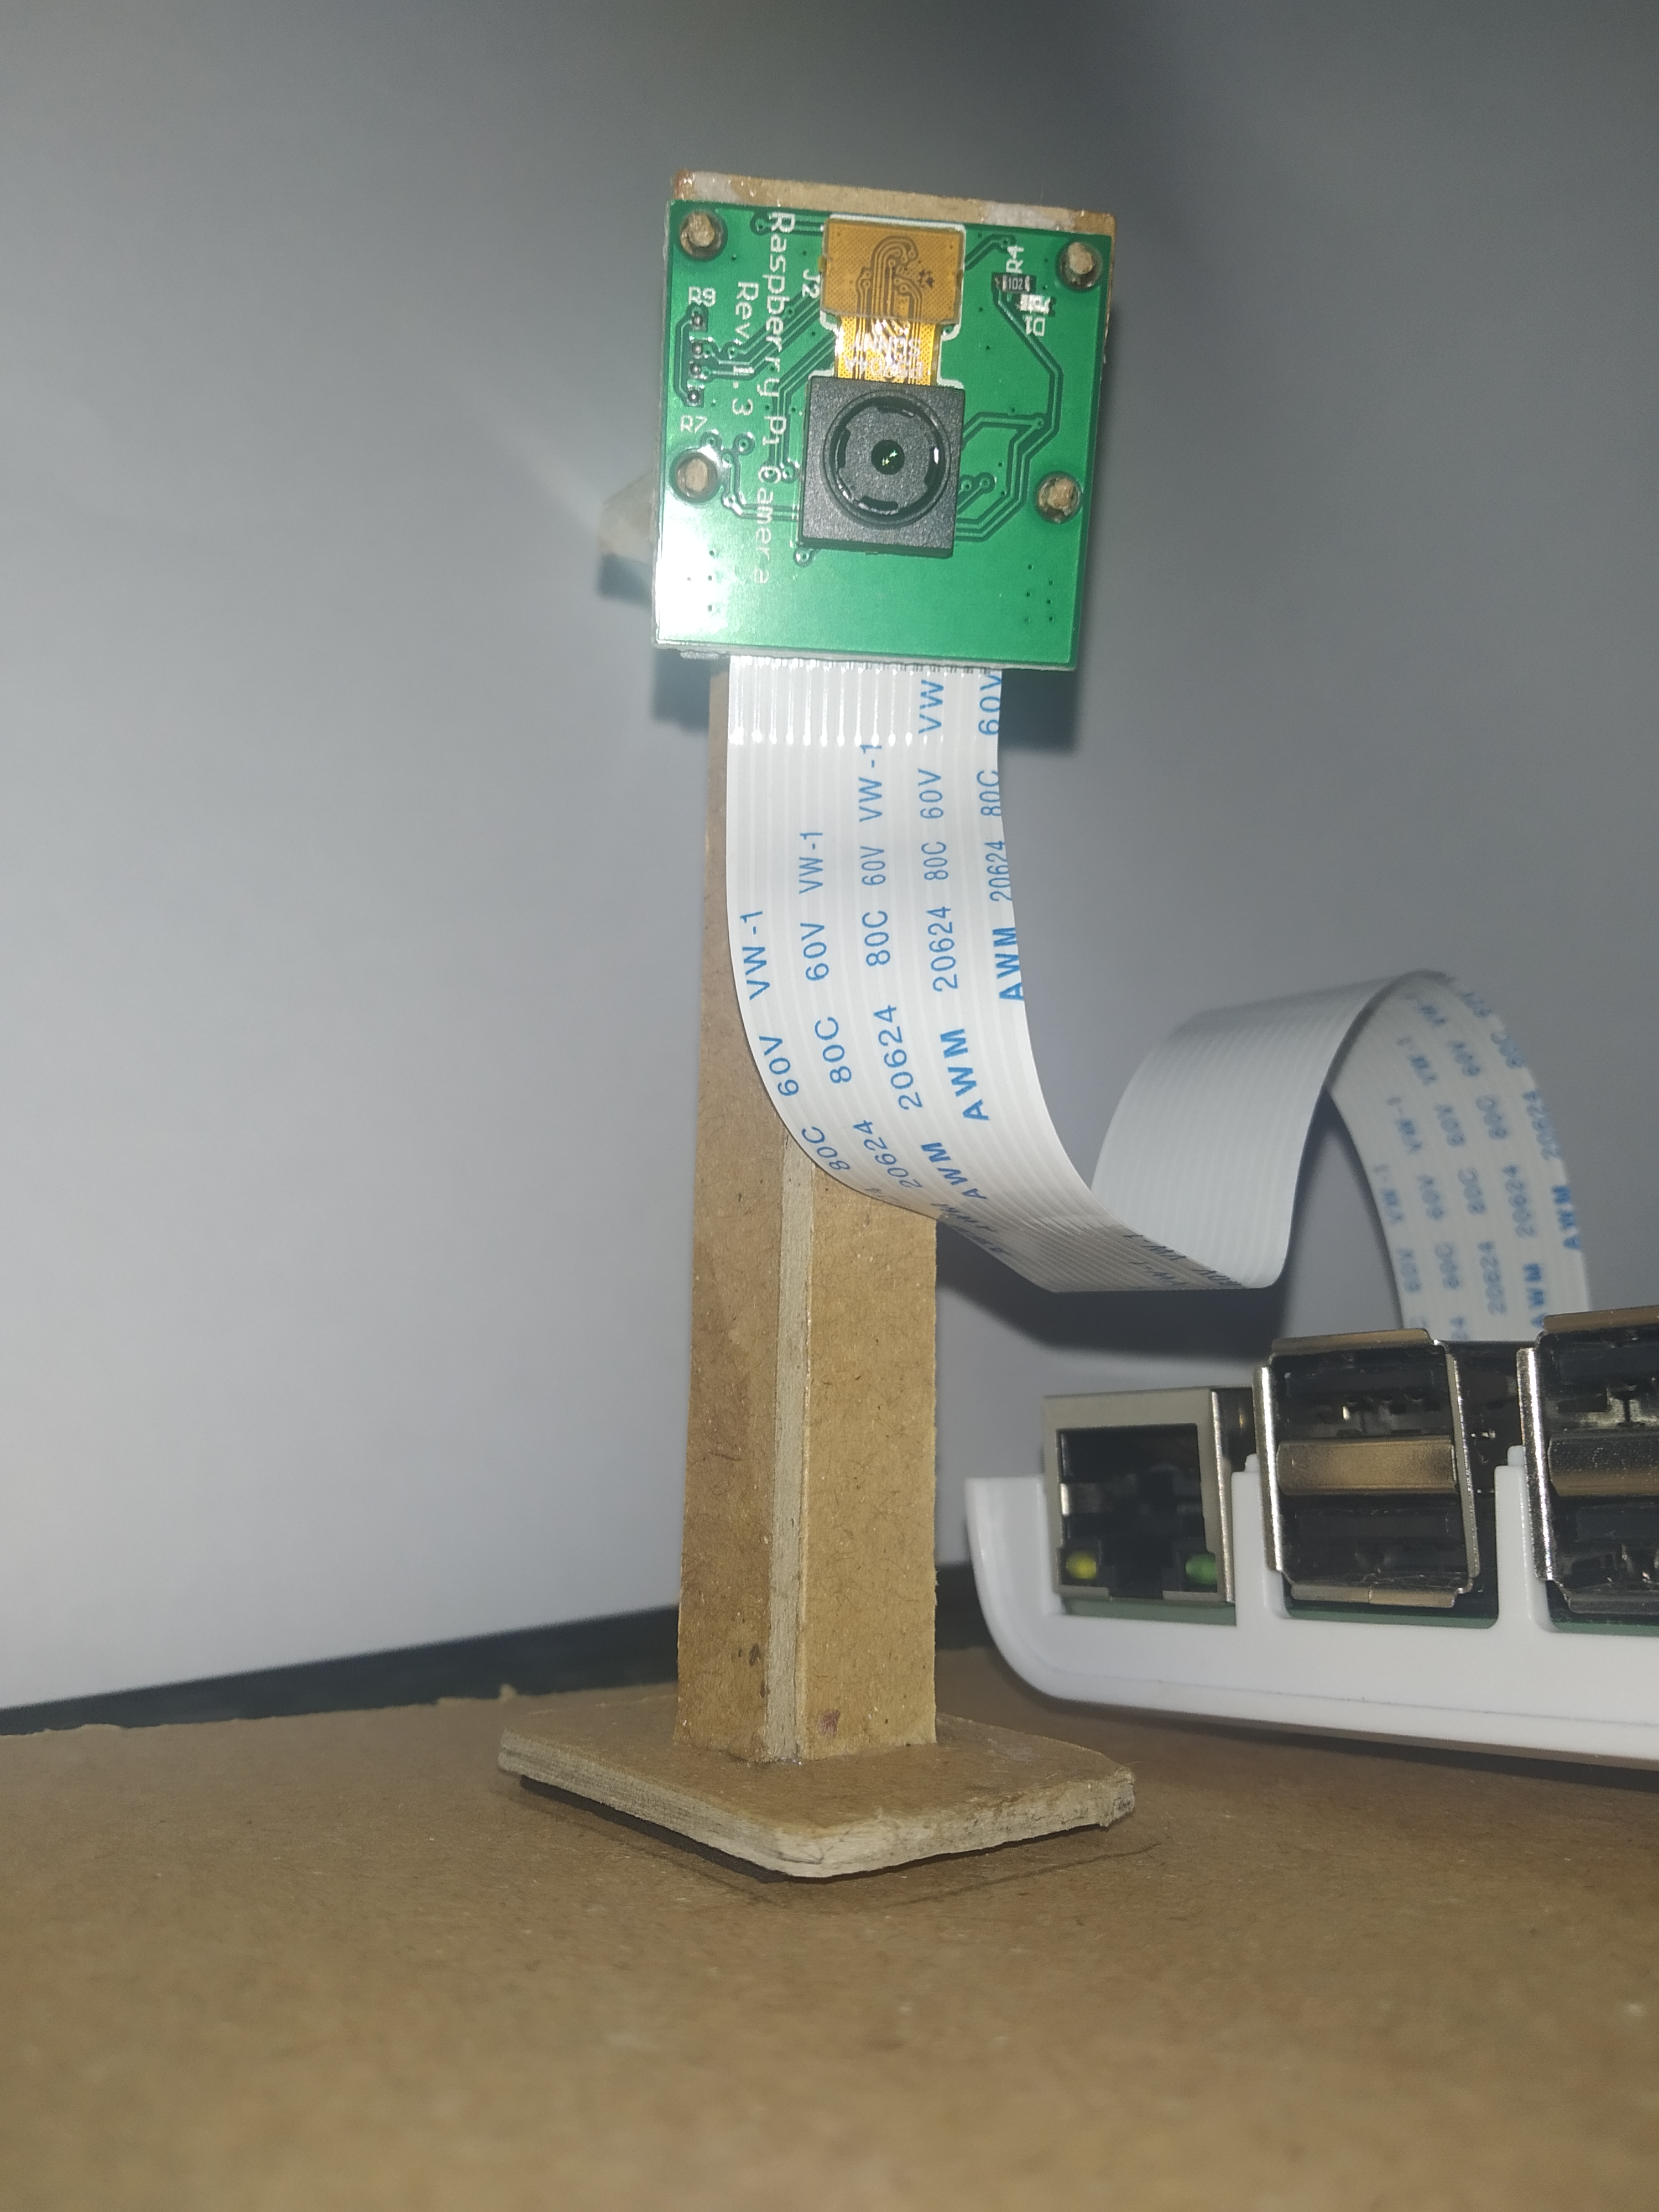
\includegraphics[height=7cm, width=0.5\textwidth, center]{images/alat-kamera.jpg}
    \caption{Hasil Rancangan Kamera}
    \label{fig:alatkamera}
\end{figure}

Pada gambar diatas merupakan rangkaian perangkat keras untuk penelitian di mana seluruh perangkat dirangkai menjadi satu rangkaian.  Gambar ~\ref{fig:alatfullmobil} merupakan hasil dari rancangan dari penelitian yang dilakukan, yang dimana masih bersifat \textit{prototype}. Pada gambar ~\ref{fig:alatservo} dapat dilihat bahwa servo digambarkan sebagai palang parkir. Pada gambar ~\ref{fig:alatultrarfid} dapat dilihat sensor ultrasonik yang akan membaca jarak dari kendaraan untuk menentukan apakah kendaraan masih ada atau sudah tidak ada dan sensor rfid untuk membaca kartu atau tag dari pengendara. Pada gambar ~\ref{fig:alatkamera} dapat dilihat kamera raspberry yang digunakan untuk mengambil nomor plat kendaraan.

\subsection{Raspberry Pi dan RFID MFRC522}
\begin{figure} [H]
    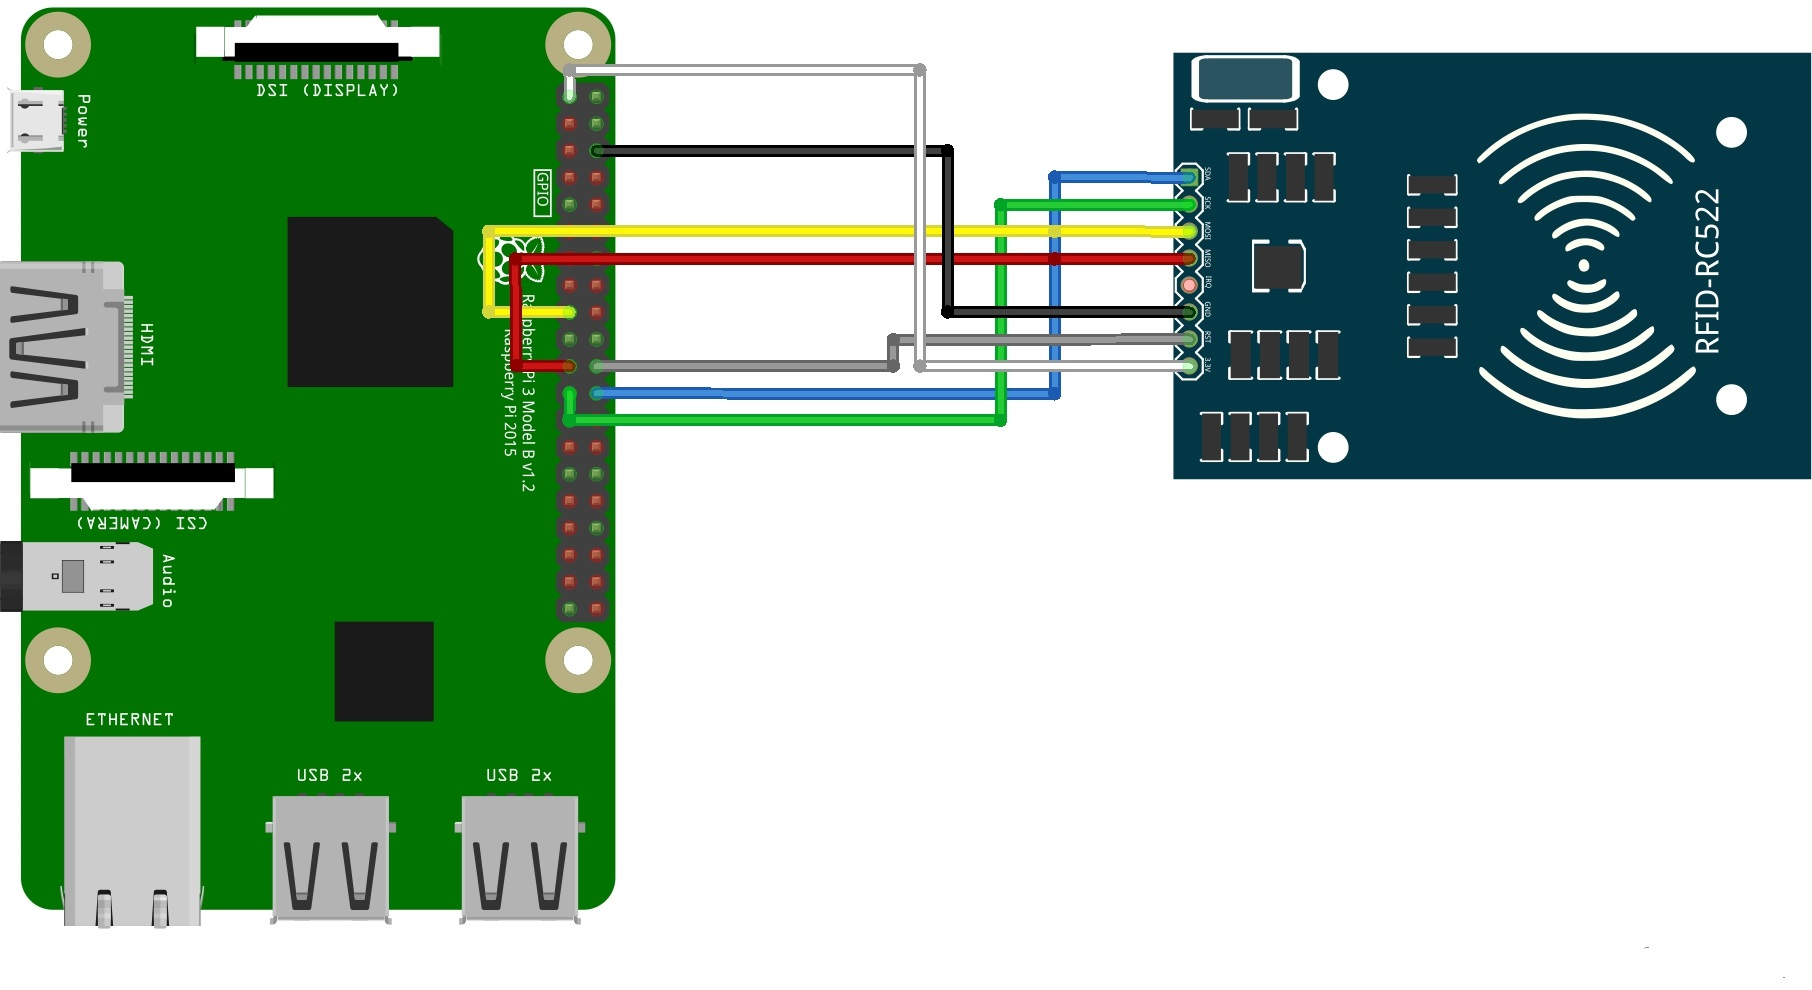
\includegraphics[width=0.85\textwidth, center]{images/skematik_rfid.jpg}
    \caption{Ragkaian Raspberry Pi dan RFID}
    \label{fig:skematikRfid}
\end{figure}

Berdasarkan gambar ~\ref{fig:skematikRfid} Menunjukkan Raspberry Pi sebagai mikrokontroler untuk menghubungkan sensor RFID yang akan membaca kartu atau tag dari pengendara. Untuk pin pada Raspberry Pi dihubungkan pada sensor RFID dapat dilihat pada tabel ~\ref{table:tableRfid}.

\begin{atable}
    \caption{Rangkaian pin RFID ke Raspberry Pi}
    \label{table:tableRfid}
    \csvreader[
        % column count = 11,
        tabular=cc,
        head to column names,
        before table=\rowcolors{2}{gray!15}{gray!30},
        table head= \rowcolor{gray!50!black} 
            \color{white} RFID & 
            \color{white} RASPBERRY PI 
            \\]
        {tables/tablerfid.csv}
        {
            RFID=\RFID, 
            RASPBERRYPI=\RASPBERRYPI}
        {
            \RFID & 
            \RASPBERRYPI}
\end{atable}

\subsection{Raspberry Pi dan HC-SR04}
\begin{figure} [H]
    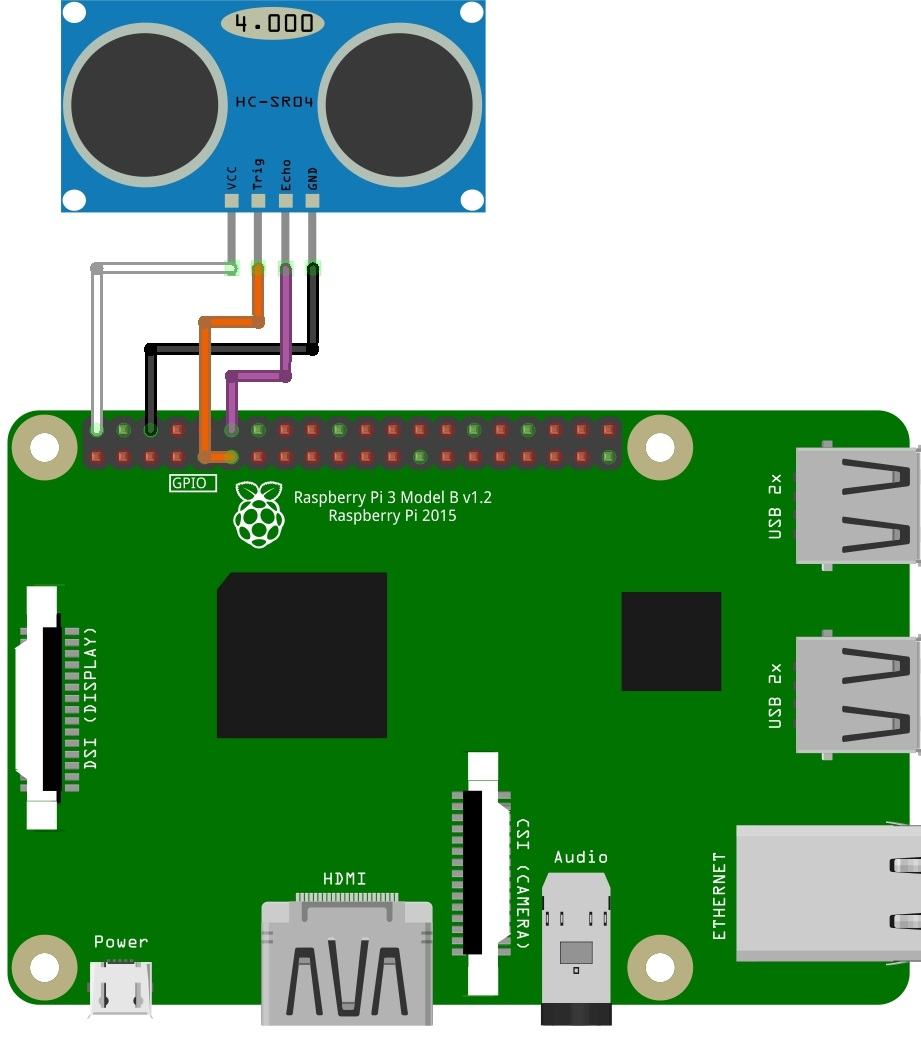
\includegraphics[height=7cm, width=0.5\textwidth, center]{images/skematik_ultra.jpg}
    \caption{Ragkaian Raspberry Pi dan Ultrasonik}
    \label{fig:skematikUltrasonik}
\end{figure}

Gambar ~\ref{fig:skematikUltrasonik} merupakan gambar rangkaian Raspberry Pi dan sensor ultrasonik. Sensor ultrasonik berfungsi sebagai indikator untuk menutup palang parkir. Apabila didepan sensor ultrasonik masih ada kendaraan, maka palang parkir masih akan terbuka, sebaliknya apabila didepan sensor sudah tidak ada kendaraan, maka palang parkir akan menutup. Sensor ultrasonik yang digunakan adalah HC-SR04 yang mempunyai 4 pin yaitu pin \textit{ground} (-), pin \textit{echo}, pin \textit{trigger}, dan pin vcc (+). Untuk pin pada Raspberry Pi dihubungkan pada sensor HC-SR04 dapat dilihat pada tabel ~\ref{table:tableUltrasonic}.

\begin{atable}
    \caption{Rangkaian pin Ultrasonik ke Raspberry Pi}
    \label{table:tableUltrasonic}
    \csvreader[
        % column count = 11,
        tabular=cc,
        head to column names,
        before table=\rowcolors{2}{gray!15}{gray!30},
        table head= \rowcolor{gray!50!black} 
            \color{white} ULTRASONIK & 
            \color{white} RASPBERRY PI 
            \\]
        {tables/tableultrasonic.csv}
        {
            ULTRASONIC=\ULTRASONIC, 
            RASPBERRYPI=\RASPBERRYPI}
        {
            \ULTRASONIC & 
            \RASPBERRYPI}
\end{atable}

\subsection{Raspberry Pi dan SG90}
\begin{figure} [H]
    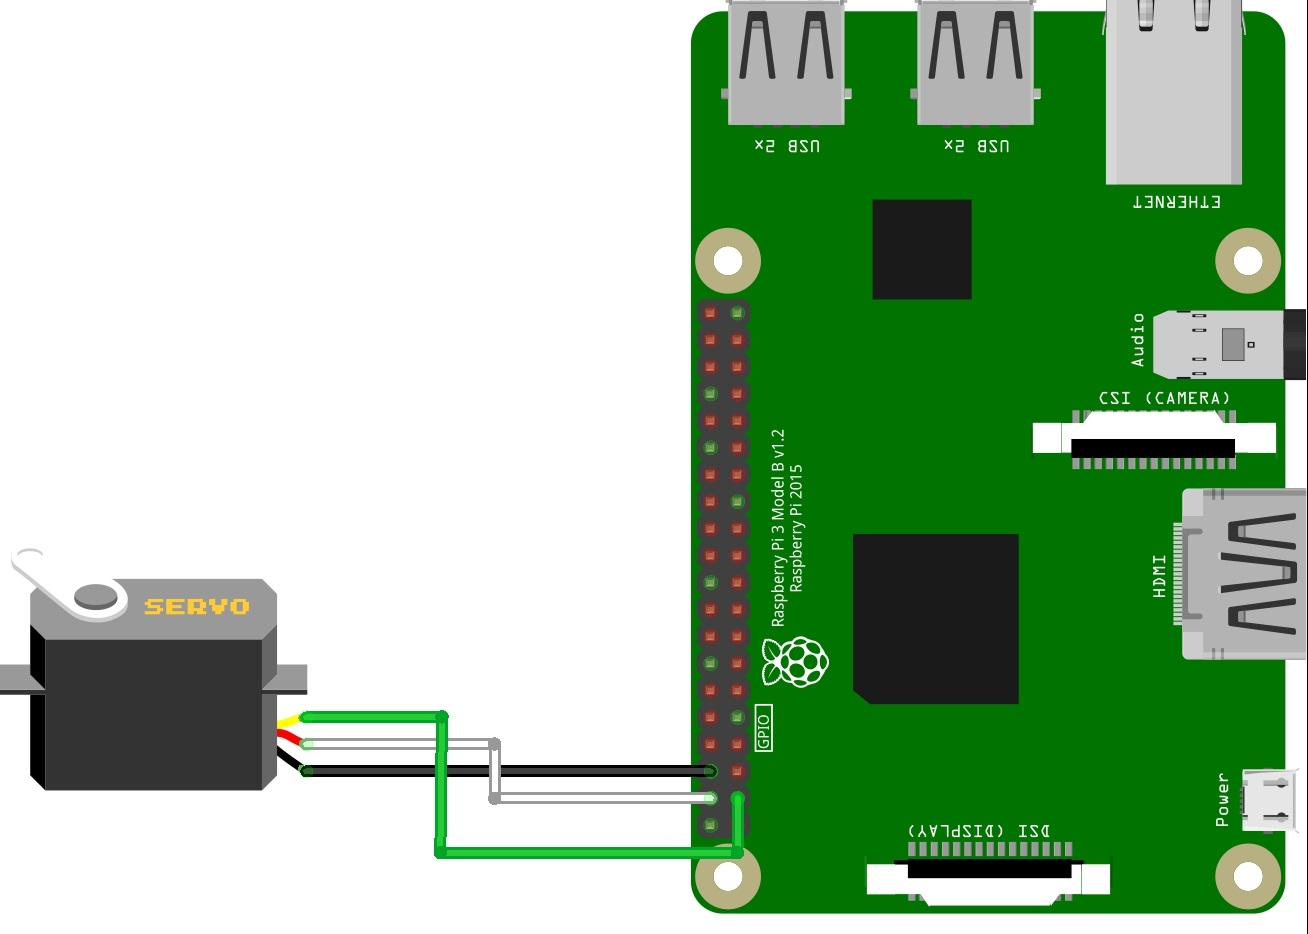
\includegraphics[height=7cm, width=0.6\textwidth, center]{images/skematik_servo.jpg}
    \caption{Ragkaian Raspberry Pi dan Servo}
    \label{fig:skematikServo}
\end{figure}

Pada penelitian ini yang akan berfungsi sebagai palang parkir adalah servo SG90. Servo yang digunakan mempunyai 3 pin yaitu pin \textit{ground} (-), pin pwm, dan pin 5v (+). Untuk pin pada Raspberry Pi dihubungkan pada servo SG90 dapat dilihat pada tabel ~\ref{table:tableServo}.

\begin{atable}
    \caption{Rangkaian pin Servo ke Raspberry Pi}
    \label{table:tableServo}
    \csvreader[
        % column count = 11,
        tabular=cc,
        head to column names,
        before table=\rowcolors{2}{gray!15}{gray!30},
        table head= \rowcolor{gray!50!black} 
            \color{white} SERVO & 
            \color{white} RASPBERRY PI 
            \\]
        {tables/tableservo.csv}
        {
            SERVO=\SERVO, 
            RASPBERRYPI=\RASPBERRYPI}
        {
            \SERVO & 
            \RASPBERRYPI}
\end{atable}

\subsection{Raspberry Pi dan Kamera Pi}

% \subsection{Hasil Perancangan Perangkat Lunak}

\section{Hasil Rancangan Aplikasi Web}

\subsection{Activity Diagram}

\subsection{Struktur \textit{Database}}
Nama \textit{database} : skripsi

Pada \textit{database} aplikasi ini, tabel dibagi menjadi 5 tabel sebagai berikut:

\begin{enumerate}[topsep=0pt,itemsep=0pt,partopsep=0pt, parsep=0pt]
    \item Tabel rfid\_tag

    Nama Tabel : rfid\_tag

    \textit{Primary Key} : id

    \begin{atable}
        \caption{rfid\_tag}
        \label{table:db_rfid_tag}
        \csvreader[
            % column count = 11,
            tabular=cc,
            head to column names,
            before table=\rowcolors{2}{gray!15}{gray!30},
            table head= \rowcolor{gray!50!black} 
                \color{white} \textit{Coloumn} & 
                \color{white} \textit{Type} 
                \\]
            {tables/db_rfid_tag.csv}
            {
                Coloumn=\Coloumn, 
                Type=\Type}
            {
                \Coloumn & 
                \Type}
    \end{atable}

    Atribut \textit{id} pada tabel rfid\_tag berfungsi sebagai kunci utama. Atribut jenis\_kendaraan digunakan untuk menentukan jenis kendaraan yang digunakan oleh pengemudi. Atribut saldo digunakan untuk menyimpan saldo dari pengemudi.

    \item Tabel tempat\_parkir

    Nama Tabel : tempat\_parkir

    \textit{Primary Key} : id

    \begin{table} [H]
        \centering
        \caption{tempat\_parkir}
        \label{table:db_tempat_parkir}
        \csvreader[
            % column count = 11,
            tabular=cc,
            head to column names,
            before table=\rowcolors{2}{gray!15}{gray!30},
            table head= \rowcolor{gray!50!black} 
                \color{white} \textit{Coloumn} & 
                \color{white} \textit{Type} 
                \\]
            {tables/db_tempat_parkir.csv}
            {
                Coloumn=\Coloumn, 
                Type=\Type}
            {
                \Coloumn & 
                \Type}
    \end{table}

    Tabel tempat\_parkir mempunyai atribut \textit{id} yang berfungsi sebagai kunci utama, atribut \textit{id} juga berfungsi sebagai nomor slot tempat parkir. Atribut jenis digunakan untuk menentukan jenis dari slot parkir. Atribut tarif digunakan sebagai tarif per jam dari slot parkir. Atribut status digunakan untuk mengetahui apakah slot sedang tersedia atau terpakai.

    \item Tabel kendaraan

    Nama Tabel : kendaraan

    \textit{Primary Key} : id

    \textit{Foreign Key} : id\_rfid\_tag

    % \begin{table} [H]
    %     \centering 
    %     \caption{kendaraan}
    %     \label{table:db_kendaraan}
    %     \csvreader[
    %         % column count = 11,
    %         tabular=cc,
    %         head to column names,
    %         before table=\rowcolors{2}{gray!15}{gray!30},
    %         table head= \rowcolor{gray!50!black} 
    %             \color{white} \textit{Coloumn} & 
    %             \color{white} \textit{Type} 
    %             \\]
    %         {tables/db_kendaraan.csv}
    %         {
    %             Coloumn=\Coloumn, 
    %             Type=\Type}
    %         {
    %             \Coloumn & 
    %             \Type}
    % \end{table}

    Tabel kendaraan mempunyai atribut \textit{id} yang berfungsi sebagai kunci utama. Atribut nomor\_plat berfungsi untuk menyimpan nomor plat pengendara. Atribut id\_rfid\_tag didapat dari tabel rfid\_tag.

    \item Tabel parkir

    Nama Tabel : parkir

    \textit{Primary Key} : id

    \textit{Foreign Key} : id\_rfid\_tag, id\_tempat\_parkir

    % \begin{table} [H]
    %     \centering
    %     \caption{parkir}
    %     \label{table:db_parkir}
    %     \csvreader[
    %         % column count = 11,
    %         tabular=cc,
    %         head to column names,
    %         before table=\rowcolors{2}{gray!15}{gray!30},
    %         table head= \rowcolor{gray!50!black} 
    %             \color{white} \textit{Coloumn} & 
    %             \color{white} \textit{Type} 
    %             \\]
    %         {tables/db_parkir.csv}
    %         {
    %             Coloumn=\Coloumn, 
    %             Type=\Type}
    %         {
    %             \Coloumn & 
    %             \Type}
    % \end{table}

    Tabel kendaraan mempunyai atribut \textit{id} yang berfungsi sebagai kunci utama. Atribut id\_rfid\_tag didapat dari tabel rfid\_tag. Atribut nomor\_plat digunakan untuk menyimpan nomor plat pengendara. Atribut id\_tempat\_parkir didapat dari tabel tempat\_parkir. Atribut waktu\_masuk digunakan untuk mencatat waktu masuk pengendara. Atribut waktu\_keluar digunakan untuk mencatat waktu keluar pengguna.

    \item Tabel \textit{reload\_id}

    Nama Tabel : reload\_id

    \textit{Primary Key} : id

    \begin{table} [H]
        \centering
        \caption{reload\_id}
        \label{table:db_reload_id}
        \csvreader[
            % column count = 11,
            tabular=cc,
            head to column names,
            before table=\rowcolors{2}{gray!15}{gray!30},
            table head= \rowcolor{gray!50!black} 
                \color{white} \textit{Coloumn} & 
                \color{white} \textit{Type} 
                \\]
            {tables/db_reload_id.csv}
            {
                Coloumn=\Coloumn, 
                Type=\Type}
            {
                \Coloumn & 
                \Type}
    \end{table}

    Tabel reload\_id mempunyai atribut \textit{id} yang berfungsi sebagai kunci utama. Atribut uid digunakan untuk menyimpan id rfid tag.

\end{enumerate}

\subsection{Tampilan Website}
    \chapter{KESIMPULAN DAN SARAN}

\section{Kesimpulan}
Berdasarkan hasil penelitian yang diuraikan pada bab IV, maka peneliti menarik beberapa kesimpulan sebagai berikut :\newline
\begin{enumerate}[topsep=0pt,itemsep=0pt,partopsep=0pt, parsep=0pt]
    \item Sistem identifikasi kendaran pada pemarkiran dengan pengenalan citra plat dan pembacaan rfid berhasil diimplementasikan.
    \item Rancangan alat yang dibuat masih bersifat \textit{prototype}. Adapun alat yang digunakan yaitu Raspberry Pi, RFID, ultrasonik, servo, dan kamera.
    \item Membuat aplikasi web sebagai \textit{user interface}. Web dibuat dengan bahasa pemrograman python dan flask sebagai \textit{framework}. Web yang dibuat memiliki beberapa fitur seperti melihat slot yang terisi dan tersedia, mendaftarkan pengguna baru, menambah saldo, dan melihat informasi mengenai slot parkir.
\end{enumerate}

\section{Saran}
Adapun saran yang diberikan kepada peneliti berikutnya apabila ingin mengembangka penelitian ini agar menjadi lebih baik adalah sebagai berikut :\newline
\begin{enumerate}[topsep=0pt,itemsep=0pt,partopsep=0pt, parsep=0pt]
    \item Melakukan penelitian dan analisis lebih lanjut pada deteksi nomor pelat kendaraan karena pada penelitian ini, peneliti masih menggunakan API dari pihak ketiga.
    \item Menambahkan fitur tambah slot parkir agar sistem parkir menjadi lebih fleksibel.
    \item Menambahkan sensor disetiap slot parkir untuk mengetahui apakah pengendara sudah parkir ditempat yang sudah ditentukan.
\end{enumerate}
    \chapter*{LAMPIRAN}

\blindtext

% \subsection*{Percobaan 1}

% \begin{table}
%     \begin{small}
%         \caption{ARM Average Blur Percobaan 1}
%         \label{table:arm-aveblur1}
%         \csvreader[
%             % column count = 11,
%             head to column names,
%             longtable=cccccccc,
%             separator=semicolon,
%             before table=\rowcolors{2}{gray!15}{gray!30},
%             table head= \rowcolor{gray!50!black} 
%                 \color{white} PID & 
%                 \color{white} VIRT & 
%                 \color{white} RES &
%                 \color{white} SHR & 
%                 \color{white} Status &  
%                 \color{white} CPU(\%) &
%                 \color{white} MEM(\%) & 
%                 \color{white} Time(s) 
%                 \\]
%             {tables/performance-test/arm-aveblur5.csv}
%             {
%                 PID=\PID, 
%                 VIRT=\VIRT, 
%                 RES=\RES,
%                 SHR=\SHR, 
%                 S=\S,
%                 CPU=\CPU,
%                 MEM=\MEM, 
%                 TIME=\TIME}
%             {
%                 \PID & 
%                 \VIRT & 
%                 \RES &
%                 \SHR & 
%                 \S &
%                 \CPU &
%                 \MEM & 
%                 \TIME}
%     \end{small}
% \end{table}
    %-----------------------------------------------------------------------------
    % End Daftar masukan untuk Bab
    %=============================================================================

    %=============================================================================
    % Daftar Pustaka
    %-----------------------------------------------------------------------------
    \addcontentsline{toc}{chapter}{DAFTAR PUSTAKA}
    \printbibliography[title={DAFTAR PUSTAKA}]
    %-----------------------------------------------------------------------------
    % End Daftar Pustaka
    %=============================================================================

\end{document}
